O Capítulo~\ref{chap:metodologia} estabeleceu os requisitos que um serviço de dados auditável deve atender e o método pelo qual a solução é avaliada. Este capítulo desenvolve a solução e a aplica ao caso estudado.

As Seções~\ref{sec:visao-geral} a~\ref{sec:banco-extraido} descrevem a arquitetura seguindo o caminho do dado. Primeiro, apresentam o que se guarda, isto é, o evento, o tempo e o referencial. Em seguida, mostram como se escreve e como se lê, como a leitura chega aos consumidores, como um terceiro confere o que recebeu e como o registro é entregue em um arquivo. A Seção~\ref{sec:implementacao} descreve a implementação, e a Seção~\ref{sec:aplicacao-sbsj}, a sua aplicação à pista do SBSJ. As Seções~\ref{sec:extensoes} e~\ref{sec:limites-arq} reúnem, respectivamente, o que foi desenhado sem ser avaliado e os limites conhecidos da arquitetura.

\section{Visão geral}\label{sec:visao-geral}

A arquitetura parte de uma ideia central. O dado primário não é o estado do aeródromo, mas a sequência de afirmações feitas sobre ele, e o estado em qualquer instante é calculado a partir dessa sequência. Essa organização corresponde ao padrão \textit{event sourcing} (Seção~\ref{sec:event-sourcing}), onde cada alteração é gravada como um evento, e os eventos nunca são alterados. O estado, então, resulta da composição dos eventos até o instante pedido.

A essa ideia soma-se a separação entre escrita e leitura (CQRS). Do lado da escrita, um único ponto de entrada valida e grava os eventos, e o que ele grava é a única fonte de verdade. Do lado da leitura, cada produto é um modelo de leitura montado a partir dos mesmos eventos, como, por exemplo, o conteúdo de uma carta ou uma tabela de distâncias declaradas. Os modelos de leitura podem ser vários, podem mudar e podem ser apagados e reconstruídos, pois não guardam nada que não esteja nos eventos.

A arquitetura tem quatro peças, apresentadas na Tabela~\ref{tab:pecas}, e cada requisito da Seção~\ref{sec:requisitos} é atendido por um mecanismo dessas peças, como resume a Tabela~\ref{tab:requisitos-mecanismos}.

\begin{table}[htbp]
    \centering
    \caption{As quatro peças da arquitetura e o seu papel em CQRS.}
    \label{tab:pecas}
    \begin{tabularx}{\linewidth}{l l X}
        \toprule
        Peça & Papel & Função \\
        \midrule
        Registro & Comandos e registro de eventos & Recebe a escrita, valida a forma e grava os eventos encadeados por \textit{hash} \\
        Tópico geral & Publicação dos eventos & Publica o registro, em ordem, fora do banco \\
        Consumidores & Modelos de leitura & Conferem a cadeia, guardam o que leram e respondem com limite explícito \\
        Banco extraído & Cópia portátil do registro & Entrega, em um arquivo, os mesmos eventos e \textit{hashes}, com visões de leitura \\
        \bottomrule
    \end{tabularx}
    \par\smallskip{\small Fonte: o autor.}
\end{table}

\begin{table}[htbp]
    \centering
    \caption{Requisitos do artefato e os mecanismos que os atendem.}
    \label{tab:requisitos-mecanismos}
    \begin{tabularx}{\linewidth}{l X l}
        \toprule
        Requisito & Mecanismo & Seção \\
        \midrule
        R1 Origem de cada valor & Autor, motivo e causa no envelope de cada evento & \ref{sec:registro} \\
        R2 Reconstrução no tempo & Registro em que só se acrescenta; tempo de transação como única linha do tempo & \ref{sec:registro}, \ref{sec:tempo} \\
        R3 Consistência entre produtos & Produtos como modelos de leitura da mesma fonte, com limite explícito e regra identificada & \ref{sec:leitura}, \ref{sec:distribuicao} \\
        R4 Mínimo de informação & Derivados calculados na leitura, gravados só se necessário& \ref{sec:leitura} \\
        R5 Posição relativa & Referencial com referentes e posições $(e, r, s, o, v)$ & \ref{sec:referencial} \\
        R6 Estrutura comum e conteúdo flexível & Envelope fixo e corpo sem esquema, achatado em linhas & \ref{sec:registro} \\
        R7 Verificação por terceiros & Cadeia de \textit{hash} sobre forma canônica pública, conferida na leitura e no arquivo & \ref{sec:escrita}, \ref{sec:verificacao} \\
        \bottomrule
    \end{tabularx}
    \par\smallskip{\small Fonte: o autor.}
\end{table}

A arquitetura não depende de um banco de eventos ou de grafos dedicado, por exemplo, um banco relacional comum é suficiente. A escolha é deliberada, pois as propriedades decorrem da forma como os dados são escritos e lidos. O banco extraído (Seção~\ref{sec:banco-extraido}) é a demonstração mais direta disso, já que as mesmas propriedades valem em um arquivo, sem servidor.

A Tabela~\ref{tab:origem} indica a origem de cada elemento da arquitetura. Um elemento \emph{adotado} é usado como descrito na sua fonte, e a contribuição está apenas na sua aplicação ao domínio. Um elemento \emph{adaptado} parte de uma base conhecida, modificada para atender aos requisitos do Capítulo~\ref{chap:metodologia}, e a modificação é descrita na última coluna. Um elemento \emph{proposto} não tem precedente direto na literatura revisada, e a coluna de base indica, quando existe, o precedente mais próximo. A contribuição do trabalho concentra-se nos elementos adaptados e propostos, o que a caracteriza como exaptação, no sentido de \citeonline{gregor2013}.

\begin{table}[htbp]
    \centering
    \caption{Origem dos elementos da arquitetura.}
    \label{tab:origem}
    \small
    \begin{tabularx}{\linewidth}{X X X}
        \toprule
        Elemento & Base & Situação neste trabalho \\
        \midrule
        Registro em que só se acrescenta; estado derivado dos eventos & \textit{event sourcing} \cite{fowler2005,kleppmann2017} & adotado \\
        Separação entre escrita e leitura & CQRS \cite{young2010} & adotado \\
        Correção por novo lançamento & livro-razão \cite{helland2016} & adotado \\
        Encadeamento por \textit{hash} sobre forma canônica & \citeonline{haber1991}; RFC~8785 & adotado \\
        Ciclo de vida \texttt{BASELINE}, \texttt{DELTA} e \texttt{VOID} & \textit{TimeSlices} do AIXM & adaptado: o temporário é o ciclo de vida de uma \textit{feature} própria \\
        Posições por referente & ISO~19148 & adaptado: duas pontas medidas; azimute e declividade nunca registrados \\
        Grupos atômicos & partidas dobradas & adaptado: sem lei de conservação, a atomicidade é imposta na escrita \\
        Consumidores sobre canal não confiável & registro ordenado e CDC \cite{kleppmann2017} & adaptado: conferência da cadeia, limite explícito e fecho de dependência \\
        Referencial endereçado pelo conteúdo e trocado por evento & endereçamento por conteúdo \cite{merkle1988} & adaptado: o referencial do referenciamento linear é um objeto imutável, e a remedição é a troca de referencial por evento \\
        Distâncias declaradas derivadas na leitura, com regra identificada & regras do Anexo~14; dados derivados \cite{kleppmann2017} & proposto \\
        Banco extraído como extrato verificável & extrato do livro-razão; resumos do SQL Ledger \cite{antonopoulos2021} & proposto \\
        \bottomrule
    \end{tabularx}
    \par\smallskip{\small Fonte: o autor.}
\end{table}

\section{O registro}\label{sec:registro}

\subsection{\textit{Features}, envelope e corpo}

Cada elemento do lado ar é uma \textit{feature}, no sentido do AIXM (Seção~\ref{sec:aixm}). São \textit{features} uma pista, uma cabeceira, uma zona de parada, uma restrição, um levantamento topográfico, o próprio aeródromo e, também, os eventos operacionais. Toda alteração de uma \textit{feature} é um evento, composto por um envelope e um corpo.

O envelope identifica o evento e indica a sua origem. Ele tem a mesma forma para todos os tipos de \textit{feature}, e é nele que se atende ao requisito de origem de cada valor (Seção~\ref{sec:req-origem}). Os seus campos são os seguintes:
\begin{itemize}
    \item \texttt{feature\_id} e \texttt{feature\_type} identificam a \textit{feature} e o seu tipo, como \texttt{airport}, \texttt{runway}, \texttt{runway\_direction}, \texttt{protect\_area}, \texttt{restriction} e \texttt{survey};
    \item \texttt{event\_type} indica o papel do evento no ciclo de vida da \textit{feature} (Seção~\ref{sec:ciclo-vida});
    \item \texttt{asserted\_by} registra quem afirma, e é obrigatório e não vazio;
    \item \texttt{reason} registra o motivo, e é obrigatório no encerramento;
    \item \texttt{caused\_by} aponta o evento que motivou este, quando houver;
    \item \texttt{owner\_ref} aponta a \textit{feature} a que esta pertence, quando houver;
    \item \texttt{grupo\_id} e \texttt{grupo\_n} aparecem somente quando o evento integra uma mudança composta por vários eventos (Seção~\ref{sec:grupos}).
\end{itemize}
\begin{figure}[htbp]
    \centering
    \begin{subfigure}{\linewidth}
        \centering
        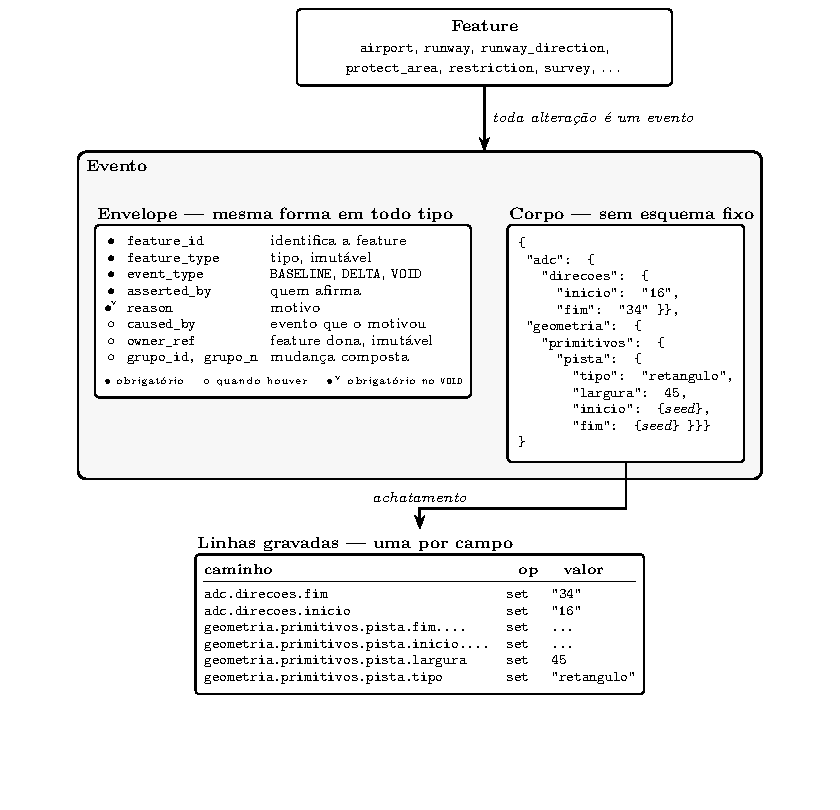
\includegraphics[page=1]{Figures/fig_evento_envelope_corpo.pdf}
        \caption{Envelope, corpo e as linhas gravadas a partir do corpo.}
        \label{fig:evento-estrutura}
    \end{subfigure}

    \bigskip
    \begin{subfigure}{\linewidth}
        \centering
        \includegraphics[page=2]{Figures/fig_evento_envelope_corpo.pdf}
        \caption{Grafo de causas, com exemplos ilustrativos.}
        \label{fig:evento-causas}
    \end{subfigure}

    \caption{Estrutura de um evento e encadeamento das causas.}
    \label{fig:evento}
    \par\smallskip{\small Fonte: o autor.}
\end{figure}
A causa só pode apontar para um evento já existente no mesmo registro e anterior ao que a declara. Por isso, as causas formam um grafo acíclico, e toda cadeia de causas termina em um evento sem causa anterior. Esse evento é uma observação, como o levantamento de uma cabeceira, ou uma decisão, como a publicação inicial de uma pista. O tipo e o dono de uma \textit{feature} também não mudam ao longo da sua vida, de modo que uma pista não se converte em pista de táxi. Uma reclassificação desse tipo é registrada como o encerramento de uma \textit{feature} seguido da criação de outra.

O corpo contém o que se afirma sobre a \textit{feature}. Ele não tem esquema fixo e consiste em um documento JSON organizado em camadas, como a camada física, com a qualidade do pavimento, e a camada de geometria, com as posições. Na gravação, o corpo é achatado em linhas, uma por campo. Cada linha é identificada pelo caminho do campo, de forma análoga ao acesso às propriedades de um objeto (por exemplo, \texttt{geometria.primitivos.pista.largura}), e registra a operação, de definição ou de remoção, e o novo valor. Esse achatamento atende ao requisito de estrutura comum e conteúdo flexível (Seção~\ref{sec:req-forma}), e dele decorrem três propriedades:
\begin{itemize}
    \item a leitura pode restringir-se a uma camada, pois um índice por caminho permite ler apenas a geometria de uma pista, sem abrir o restante do corpo;
    \item um campo ausente distingue-se de um campo nulo, já que o primeiro não foi informado e o segundo foi informado como vazio;
    \item um evento de alteração grava apenas os campos que mudam, e a diferença entre dois instantes é a lista desses campos, com os valores anteriores e posteriores.
\end{itemize}

\subsection{Ciclo de vida}\label{sec:ciclo-vida}

Há três tipos de evento, com nomes emprestados do AIXM:
\begin{itemize}
    \item \texttt{BASELINE} cria a \textit{feature} com o corpo completo, ou a recria após um encerramento;
    \item \texttt{DELTA} altera campos do corpo e grava apenas os caminhos alterados, sem repetir o estado anterior, que já está nos eventos precedentes;
    \item \texttt{VOID} encerra o ciclo de vida da \textit{feature} e exige um motivo. Não se trata de exclusão nem de anulação de um evento anterior; o histórico permanece, e a \textit{feature} apenas deixa de existir a partir daquele instante.
\end{itemize}

O significado desses tipos é mais simples que no AIXM, pois não há distinção estrutural entre alteração permanente e temporária. Uma interdição temporária, por exemplo, é uma \textit{feature} de restrição, com a pista como dona, criada por um \texttt{BASELINE} e encerrada por um \texttt{VOID}, e a sua duração resulta da sequência de eventos. Operações como substituir, dividir ou fundir \textit{features} também não são primitivas, e se compõem de sequências de \texttt{BASELINE} e \texttt{VOID}. A Figura~\ref{fig:ciclo-vida} mostra os estados de uma \textit{feature} e as transições que a escrita recusa.

\begin{figure}[htbp]
    \centering
    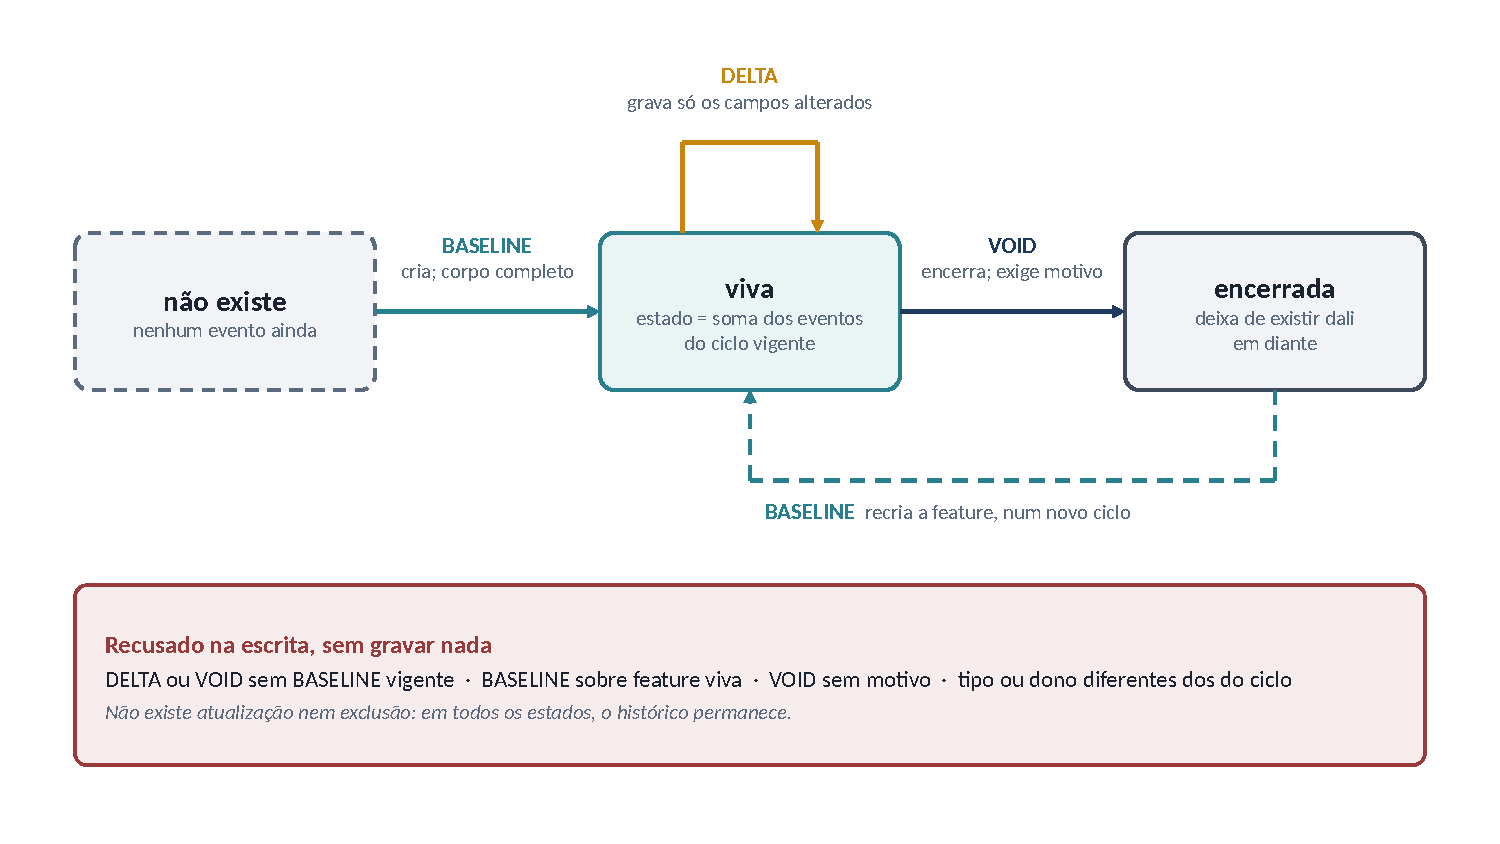
\includegraphics[width=\linewidth]{Figures/fig_ciclo_vida.pdf}
    \caption{Ciclo de vida de uma \textit{feature} e as transições que a escrita recusa.}
    \label{fig:ciclo-vida}
    \par\smallskip{\small Fonte: o autor.}
\end{figure}


\subsection{Grupos}\label{sec:grupos}

Algumas mudanças exigem mais de um evento. A carga de uma edição do AIP, por exemplo, cria de uma só vez o aeródromo, a pista, as cabeceiras e a zona de parada. Uma leitura feita no meio dessa carga mostraria a pista sem a zona de parada e calcularia uma ASDA igual à TORA, sem nenhum erro aparente. Para evitar esse estado intermediário, a arquitetura define o grupo, um conjunto de dois ou mais eventos gravados juntos, ou todos ou nenhum, contíguos no registro e no mesmo instante.

Cada evento do grupo leva no envelope o \texttt{grupo\_id}, que é o identificador do primeiro evento, e o \texttt{grupo\_n}, que é o número de eventos do grupo. O primeiro campo registra quais eventos formam uma mesma mudança, o que o instante comum, por si só, não garante. O segundo permite a quem lê saber se já recebeu o grupo inteiro. Uma leitura cujo limite caia dentro de um grupo recua até antes dele, de modo que nenhum corte mostra uma mudança pela metade (Seção~\ref{sec:distribuicao}).

O grupo cumpre o papel do lançamento em um livro-razão de partidas dobradas, no qual as partidas de uma transferência entram juntas e o livro nunca mostra o débito sem o crédito. Há, contudo, uma diferença. Na contabilidade, as partidas de um lançamento somam zero, e uma transferência incompleta se denuncia sozinha. Aqui não há lei de conservação, e uma pista sem zona de parada é um estado plausível. A atomicidade, por isso, não pode depender de uma conferência posterior.

\section{Tempo}\label{sec:tempo}

A arquitetura usa uma única linha do tempo, o tempo de transação, isto é, o instante em que cada evento foi registrado (Seção~\ref{sec:bitemporal}). Os motivos dessa escolha estão na Seção~\ref{sec:req-tempo}. Cada aeródromo tem a sua cadeia de eventos, e cada cadeia tem um relógio que só avança, de modo que nada se escreve no passado. A Figura~\ref{fig:linha-tempo} ilustra a linha do tempo de duas \textit{features}.

\begin{figure}[h]
    \centering
    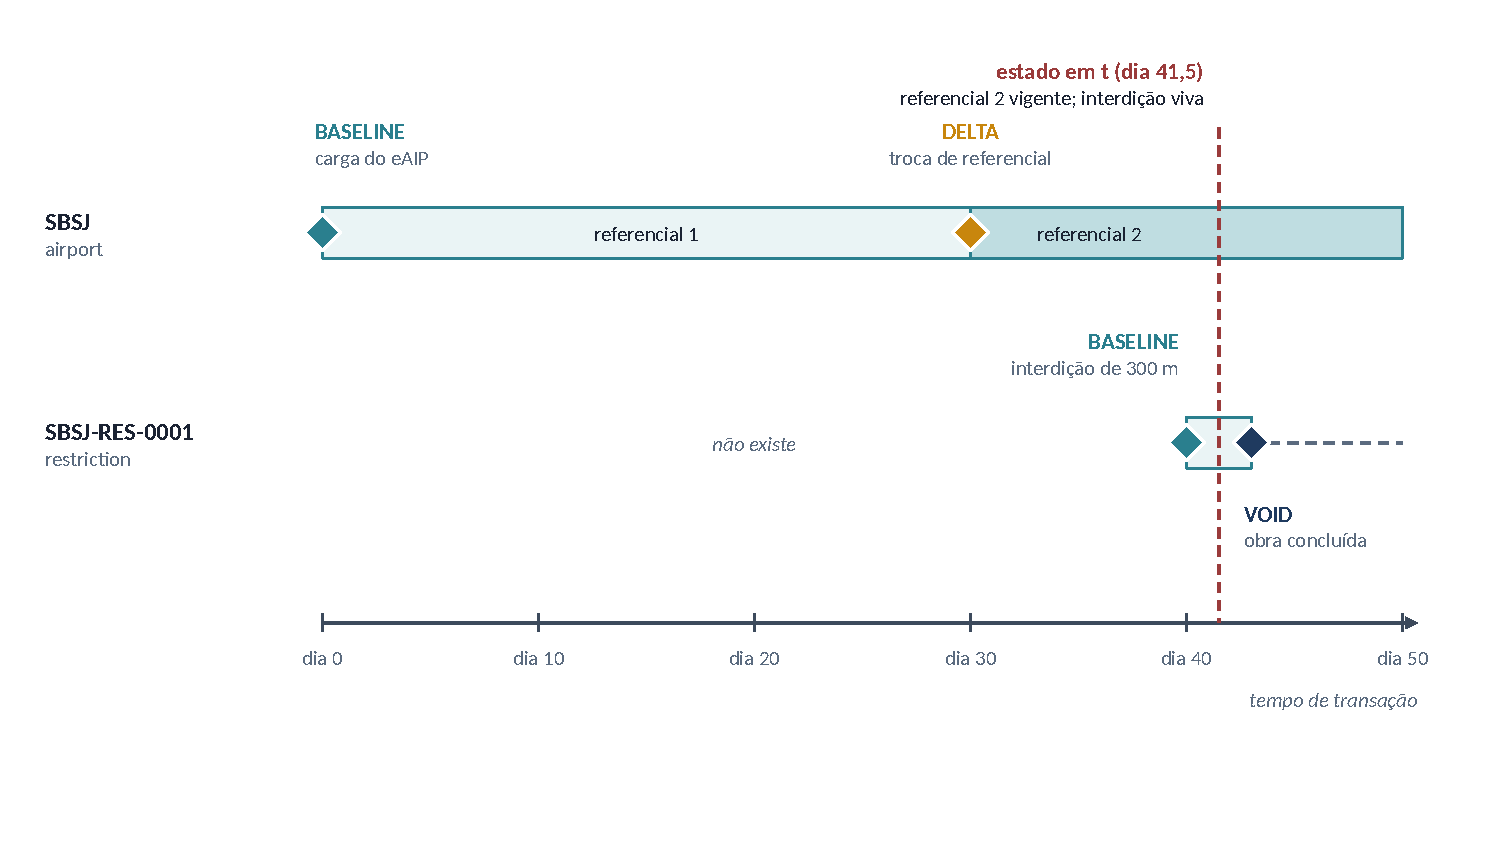
\includegraphics[width=\linewidth]{Figures/fig_ciclo_vida_tempo.pdf}
    \caption{Linha do tempo de duas \textit{features} e o estado em um instante $t$.}
    \label{fig:linha-tempo}
    \par\smallskip{\small Fonte: o autor.}
\end{figure}


O identificador do evento (\texttt{event\_id}) segue o esquema Snowflake \cite{twitter2010snowflake}, com 41 \textit{bits} de milissegundos desde uma data arbitrária, 10 de partição e 12 de sequência (Figura~\ref{fig:snowflakeid}). O instante é extraído do próprio identificador, cuja ordem coincide com a do tempo, e a escrita recusa um evento anterior ao último gravado.

\begin{figure}[htbp]
    \centering
    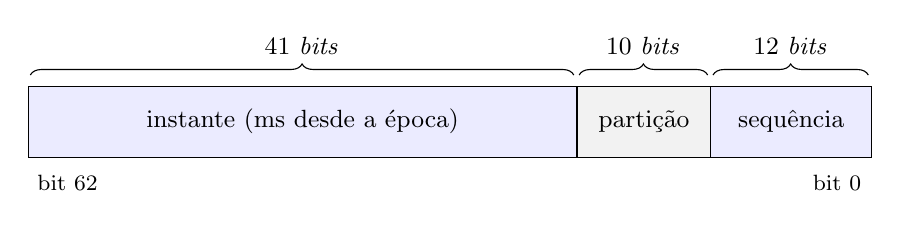
\begin{tikzpicture}[x=0.17cm, y=1cm, font=\small,
        campo/.style={draw, minimum height=0.9cm, anchor=south west, inner sep=0pt}]
        % larguras proporcionais ao número de bits: 41 | 10 | 12
        \node[campo, fill=blue!8,  minimum width=41*0.17cm] at (0,0)  {instante (ms desde a época)};
        \node[campo, fill=gray!10, minimum width=10*0.17cm] at (41,0) {partição};
        \node[campo, fill=blue!8,  minimum width=12*0.17cm] at (51,0) {sequência};
        \foreach \a/\b/\n in {0/41/41, 41/51/10, 51/63/12} {
            \draw[decorate, decoration={brace, amplitude=4pt}] (\a+0.2,1.05) -- (\b-0.2,1.05)
                node[midway, above=4pt] {\n\ \textit{bits}};
        }
        \node[anchor=north west, font=\footnotesize] at (0,-0.1) {bit 62};
        \node[anchor=north east, font=\footnotesize] at (63,-0.1) {bit 0};
    \end{tikzpicture}
    \caption{Composição do identificador de um evento.}
    \label{fig:snowflakeid}
    \par\smallskip{\small Fonte: o autor.}
\end{figure}

Na leitura, o instante $t$ pode ser uma data e hora ou um \texttt{event\_id}, e ambos são convertidos em um limite superior de identificador. Uma data e hora corresponde ao maior identificador possível naquele milissegundo, e um \texttt{event\_id} distingue eventos do mesmo milissegundo, como os de um grupo. Toda consulta se reduz, assim, a ``tudo até o evento $N$''.

A extensão para dois eixos de tempo está entre as propostas da Seção~\ref{sec:extensoes}, no qual uma data alegada por quem escreve, como a data de uma medição ou a entrada em vigor de uma emenda AIRAC, é conteúdo do corpo. 

\section{Referencial e posição}\label{sec:referencial}

\subsection{O referencial}

O requisito de posição relativa (Seção~\ref{sec:req-posicao}) é atendido por um referencial, documento que declara os referentes, isto é, os pontos medidos em que as posições se apoiam, e os elementos lineares entre eles. No SBSJ, o referencial tem dois referentes georreferenciados, as cabeceiras THR16 e THR34, e um elemento linear entre elas, RWY\_16\_34. Cada referente tem latitude, longitude, elevação, ondulação geoidal e fonte, e o datum é o SIRGAS2000. A Figura~\ref{fig:referencial-sbsj} mostra esse referencial.

\begin{figure}[htbp]
    \centering
    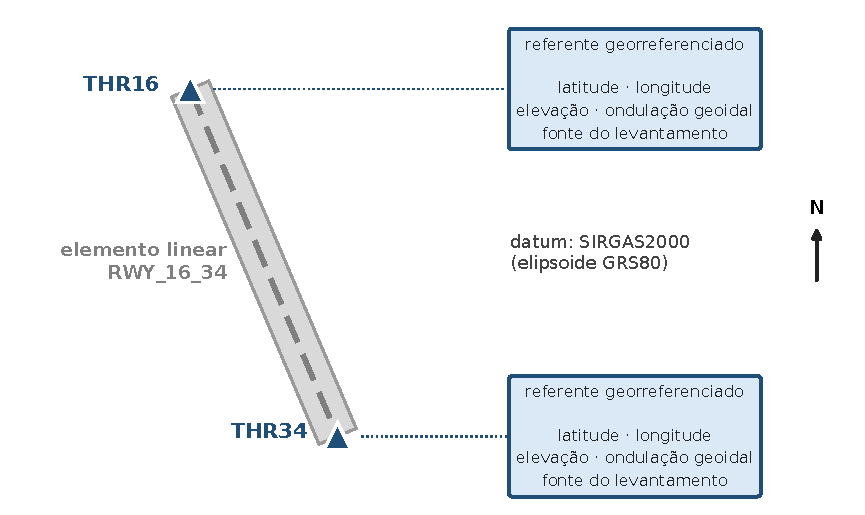
\includegraphics[width=0.85\linewidth]{Figures/fig-referencial-sbsj.pdf}
    \caption{Referencial do SBSJ: as cabeceiras THR16 e THR34 como referentes georreferenciados e o elemento linear RWY\_16\_34 entre elas.}
    \label{fig:referencial-sbsj}
    \par\smallskip{\small Fonte: o autor.}
\end{figure}

A publicação de um referencial deve seguir as seguintes regras (Figura~\ref{fig:regras-referencial}), sob pena de ser rejeitada:
\begin{itemize}
    \item cada referente deve ser definido por exatamente um dos seguintes
    métodos: por georreferenciamento, com latitude e longitude, ou por
    posicionamento relativo a outro referente, medido ao longo de um
    elemento linear a partir de uma de suas pontas;
    \item as relações entre referentes não podem formar ciclos, e todo
    encadeamento deve terminar em um referente georreferenciado;
    \item todo elemento linear deve possuir exatamente duas pontas distintas;
    \item o posicionamento relativo de um referente exige um elemento linear,
    pois, sem ele, não há uma direção definida para determinar o afastamento
    em relação ao referente de origem.
\end{itemize}

\begin{figure}[htbp]
    \centering
    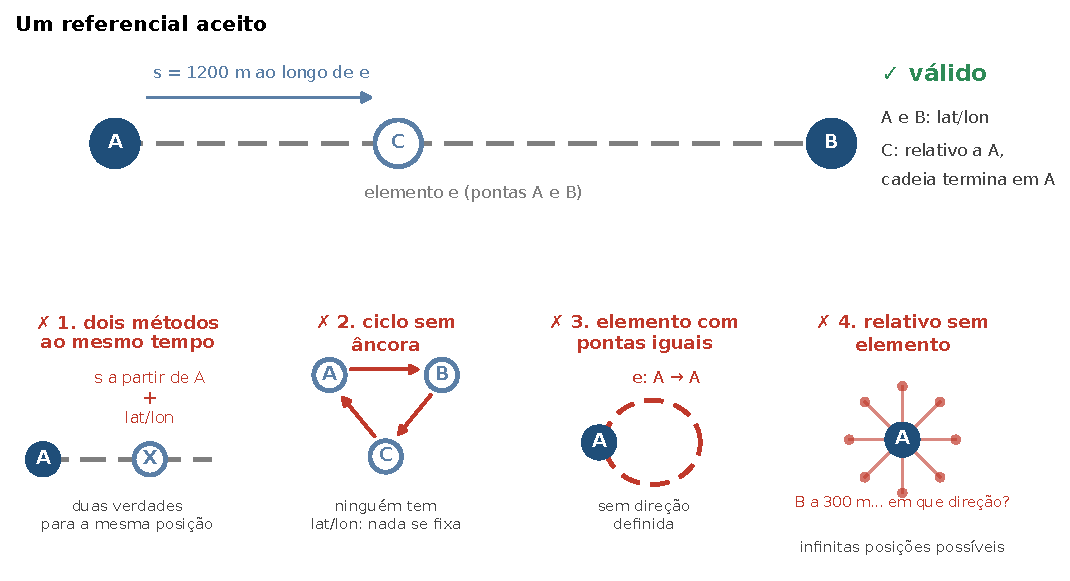
\includegraphics[width=\linewidth]{Figures/fig-regras-referencial.pdf}
    \caption{Exemplo de referencial aceito e um caso de rejeição para cada regra de publicação.}
    \label{fig:regras-referencial}
    \par\smallskip{\small Fonte: o autor.}
\end{figure}

O número de referentes é livre. Um aeroporto com várias pistas teria um elemento linear por eixo, e os referentes de uma pista poderiam ser independentes dos de outra. Essa configuração não é avaliada neste trabalho.

O referencial é endereçado pelo conteúdo, ou seja, o seu identificador (\texttt{ref\_id}) é o \textit{hash} SHA-256 da sua forma canônica (Seção~\ref{sec:escrita}). Dois referenciais com o mesmo conteúdo têm o mesmo identificador, e nenhum pode ser alterado sem mudar de identificador. O referencial vigente é um campo do corpo da \textit{feature} \texttt{airport}, e trocá-lo é um \texttt{DELTA} nessa \textit{feature}. A escrita recusa a troca se alguma posição gravada ficar sem apoio no novo referencial.

\subsection{Posições}

Toda posição que não seja um referente é gravada como uma \textit{seed}, segundo o referenciamento linear da ISO~19148 (Equação~\ref{eq:lrs}). O elemento linear $e$ fornece a direção, e o referente $r$, sempre sobre o elemento, fornece a origem. A distância $s$ é positiva no sentido da outra ponta do elemento, e o afastamento lateral $o$ é positivo à direita de quem percorre o elemento no sentido de $s$. A altitude da posição é
\begin{equation}
    z(p) = z_r + v
    \label{eq:altitude-posicao}
\end{equation}
em que $z_r$ é a altitude do referente e $v$ o afastamento vertical. Os componentes da \textit{seed} estão ilustrados na Figura~\ref{fig:seed-lrs}.

\begin{figure}[htbp]
    \centering
    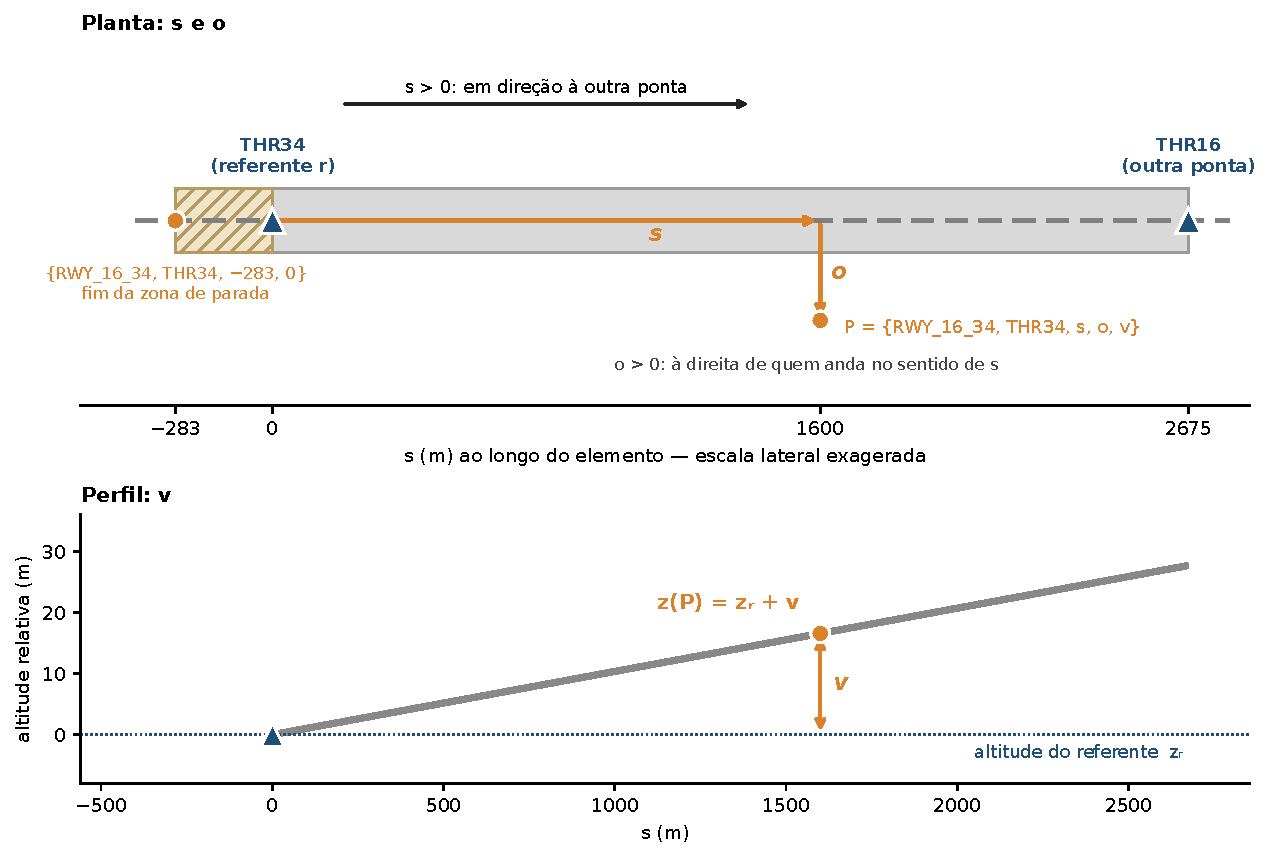
\includegraphics[width=\linewidth]{Figures/fig-seed-lrs.pdf}
    \caption{Componentes de uma \textit{seed}: em planta, a distância $s$ e o afastamento lateral $o$; em perfil, o afastamento vertical $v$ a partir da altitude do referente. A escala lateral da planta está exagerada.}
    \label{fig:seed-lrs}
    \par\smallskip{\small Fonte: o autor.}
\end{figure}

A zona de parada do SBSJ, por exemplo, termina em $\{\mathrm{RWY\_16\_34},\, \mathrm{THR34},\, -283,\, 0\}$, isto é, 283~m para fora da cabeceira~34, sobre o eixo. Um afastamento vertical ausente significa ``não informado'', e não zero. A posição continua definida no plano, mas a sua altitude não. Em uma pista em rampa, um zero implícito atribuiria à posição a altitude do referente, o que estaria errado. A Figura~\ref{fig:afastamento-vertical-ausente} ilustra a diferença.

\begin{figure}[htbp]
    \centering
    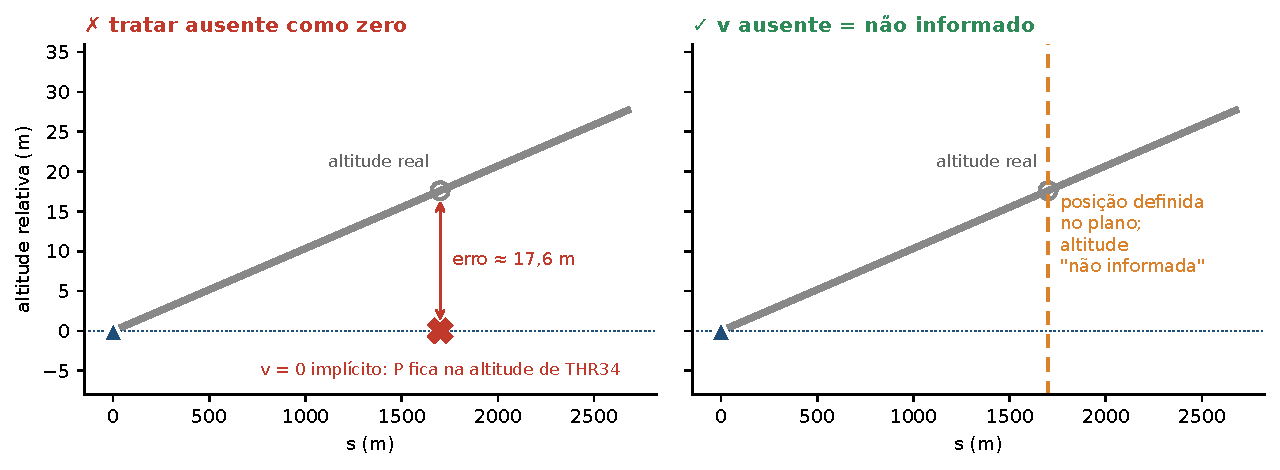
\includegraphics[width=\linewidth]{Figures/fig-afastamento-vertical-ausente.pdf}
    \caption{Afastamento vertical ausente: tratado como zero, atribui à posição a altitude do referente; tratado como não informado, mantém a posição definida apenas no plano.}
    \label{fig:afastamento-vertical-ausente}
    \par\smallskip{\small Fonte: o autor.}
\end{figure}

O azimute do eixo é calculado pela geodésica entre as duas pontas do elemento e recalculado ao longo do caminho, razão pela qual a posição depende do elemento, e não apenas do referente. Pelo mesmo motivo, a declividade do eixo decorre da diferença de altitude entre as pontas.

\subsection{Escolha dos referentes}

A arquitetura não permite registrar um azimute. A alternativa seria posicionar a pista a partir de um único referente e do azimute do eixo, que passaria a ser uma premissa. Nesse caso, um erro angular $\delta\theta$ produziria, a uma distância $s$, um erro lateral aproximado de
\begin{equation}
    \varepsilon_\perp \approx s \cdot \delta\theta
    \label{eq:erro-angular}
\end{equation}


Na pista do SBSJ, um erro de $0{,}01^\circ$ no azimute corresponde a aproximadamente 0,47~m na cabeceira oposta (Figura~\ref{fig:erro-angular}). Com as duas cabeceiras como pontas do eixo, esse erro não existe como premissa, porque o azimute decorre das posições medidas. O mesmo vale na vertical. Uma declividade registrada como premissa propagaria o seu erro com a distância, ao passo que, com as altitudes das duas pontas medidas, ela é apenas um valor derivado.

\begin{figure}[htbp]
    \centering
    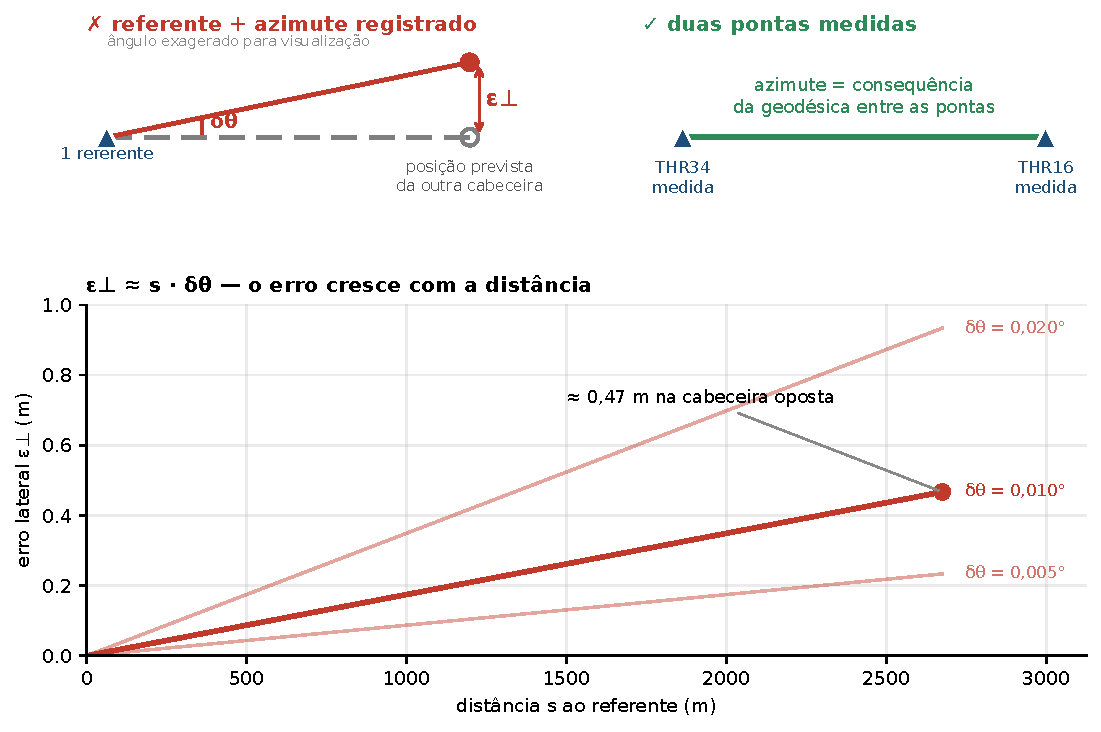
\includegraphics[width=\linewidth]{Figures/fig-erro-angular.pdf}
    \caption{Posicionamento por um referente e um azimute registrado, comparado ao posicionamento por duas pontas medidas, e o erro lateral $\varepsilon_\perp \approx s\,\delta\theta$ ao longo da pista do SBSJ. O ângulo do esquema superior está exagerado.}
    \label{fig:erro-angular}
    \par\smallskip{\small Fonte: o autor.}
\end{figure}

Referentes adicionais, como marcos geodésicos ou pontos de mudança de greide do perfil longitudinal, reduzem a distância entre uma posição e o ponto medido mais próximo (Figura~\ref{fig:referentes-adicionais}), mas também oferecem redundância. A distância calculada entre dois referentes pode ser comparada com a medida em campo, e uma divergência indica que uma das medições precisa ser verificada.

\begin{figure}[htbp]
    \centering
    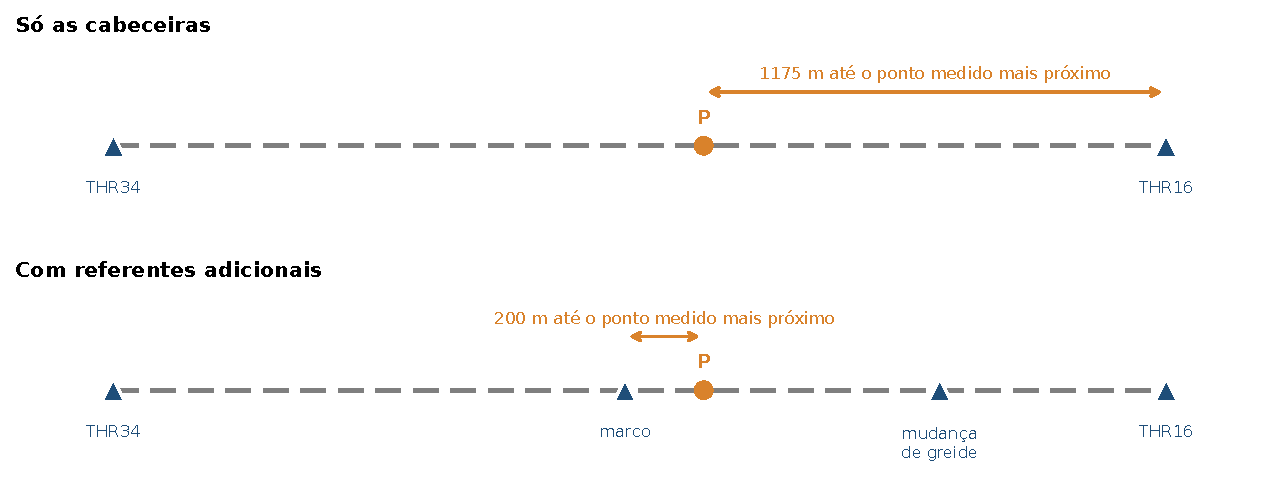
\includegraphics[width=\linewidth]{Figures/fig-referentes-adicionais.pdf}
    \caption{Efeito de referentes adicionais sobre a distância entre uma posição e o ponto medido mais próximo. As posições do marco e da mudança de greide são ilustrativas.}
    \label{fig:referentes-adicionais}
    \par\smallskip{\small Fonte: o autor.}
\end{figure}

\subsection{Plano e altitude}\label{sec:plano-altitude}

A arquitetura trata o plano e a altitude separadamente, como a geodésia faz com a planimetria e a altimetria. No plano, $s$ e $o$ são distâncias geodésicas sobre o elipsoide GRS80, adotado pelo SIRGAS2000, e não distâncias sobre uma projeção cartográfica (Seção~\ref{sec:geodesia}). Na carta de aeródromo do SBSJ, por exemplo, a diferença entre o norte da quadrícula e o norte verdadeiro é de cerca de $0{,}33^\circ$. A geodésica sobre o elipsoide dispensa essas convenções e serve, por isso, de régua comum a qualquer produto. Na altitude, a referência é a do próprio referente, e $v$ é uma diferença de altitude a partir dele.

Essa separação tem uma consequência que precisa ser declarada. Um comprimento calculado sobre o elipsoide não é o comprimento medido sobre o pavimento, e as reduções de altitude e de inclinação os separam (Equações~\ref{eq:reducao-altitude} e~\ref{eq:reducao-inclinacao}). Na pista do SBSJ, a uma altitude de cerca de 630~m e com desnível de 27,7~m, as duas reduções somam cerca de 0,4~m em 2675~m, sendo aproximadamente 0,26~m devidos à altitude e 0,14~m à inclinação (Figura~\ref{fig:plano-altitude}). A arquitetura fixa como convenção o comprimento sobre o elipsoide e a declara como parte da regra de derivação, para que dois produtos nunca misturem convenções. Quando um produto precisar das correções, elas são outros valores derivados, calculados a partir das altitudes dos referentes.

\begin{figure}[htbp]
    \centering
    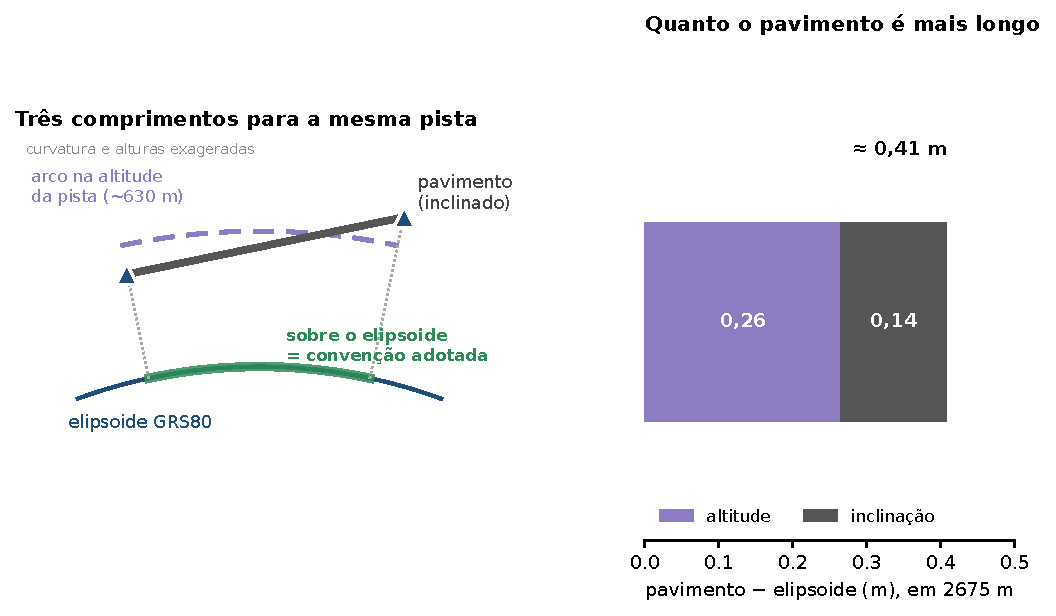
\includegraphics[width=\linewidth]{Figures/fig-plano-altitude.pdf}
    \caption{Comprimento sobre o elipsoide, na altitude da pista e sobre o pavimento inclinado, e as reduções de altitude e de inclinação na pista do SBSJ. Curvatura e alturas do esquema estão exageradas.}
    \label{fig:plano-altitude}
    \par\smallskip{\small Fonte: o autor.}
\end{figure}

\subsection{Remedição como evento}

Como nenhuma \textit{seed} guarda coordenadas nem comprimentos, a remedição de uma cabeceira é registrada em três passos (Figura~\ref{fig:remedicao-evento}). O primeiro é um evento que registra o levantamento, como \textit{feature} própria. O segundo é a publicação de um referencial com a nova posição da cabeceira. O terceiro é um \texttt{DELTA} na \textit{feature} \texttt{airport} que troca o \texttt{ref\_id}, com causa no levantamento. A pista, a zona de parada e as distâncias declaradas acompanham a mudança na leitura seguinte, e o histórico mostra por que mudaram.

\begin{figure}[htbp]
    \centering
    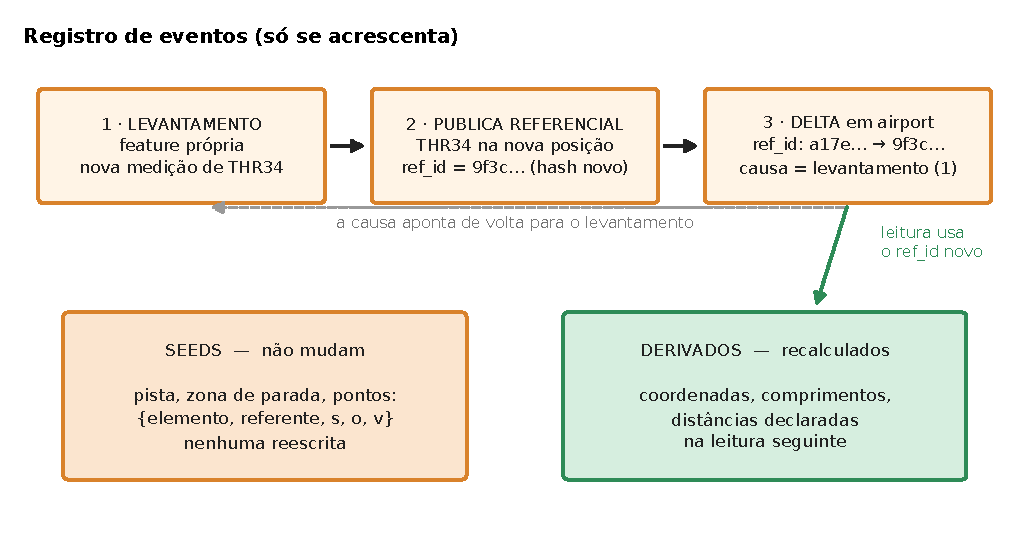
\includegraphics[width=\linewidth]{Figures/fig-remedicao-evento.pdf}
    \caption{Remedição de uma cabeceira como sequência de eventos: as \textit{seeds} permanecem inalteradas e os valores derivados são recalculados a partir do novo referencial. Os identificadores são ilustrativos.}
    \label{fig:remedicao-evento}
    \par\smallskip{\small Fonte: o autor.}
\end{figure}

\subsection{Geometria}

A geometria das \textit{features} também é derivada. Ela é gerada a partir das \textit{seeds}, com primitivos simples (ponto, retângulo e coroa), em um plano local em metros centrado em um dos referentes (Figura~\ref{fig:geometria-derivada}). A geometria serve para desenhar a carta a partir do registro, mas não integra as propriedades avaliadas.

\begin{figure}[htbp]
    \centering
    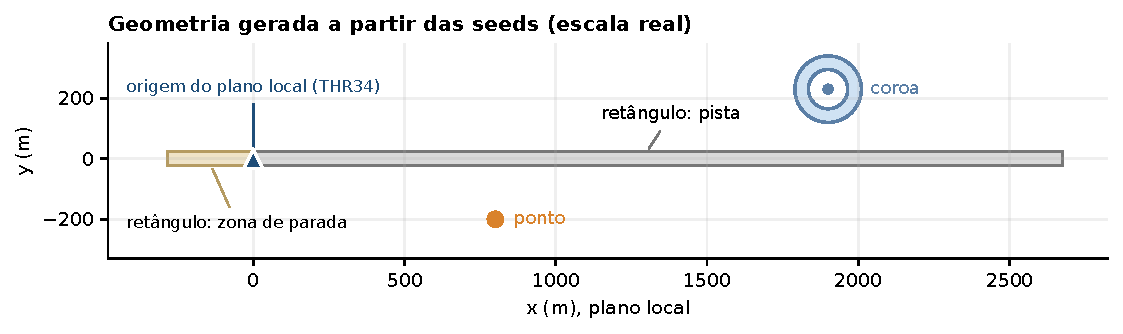
\includegraphics[width=\linewidth]{Figures/fig-geometria-derivada.pdf}
    \caption{Geometria gerada a partir das \textit{seeds} no plano local com origem em THR34. O ponto e a coroa são ilustrativos.}
    \label{fig:geometria-derivada}
    \par\smallskip{\small Fonte: o autor.}
\end{figure}

\section{A escrita}\label{sec:escrita}

\subsection{Forma e domínio}

A escrita tem apenas duas operações, a gravação de um evento e a gravação de um grupo. Ambas recusam, sem gravar nada, tudo o que viola a forma do registro, isto é:
\begin{itemize}
    \item tipo de evento inválido;
    \item \texttt{DELTA} ou \texttt{VOID} sem \texttt{BASELINE} vigente;
    \item \texttt{BASELINE} sobre \textit{feature} viva;
    \item envelope alterado;
    \item \texttt{VOID} sem motivo;
    \item autor vazio;
    \item caminho malformado, remoção de campo ausente e campo que seja ao mesmo tempo valor e prefixo de outro;
    \item causa que aponte para evento inexistente;
    \item posição que aponte para referente inexistente;
    \item troca de referencial que deixe alguma posição sem apoio.
\end{itemize}
Se qualquer evento de um grupo for recusado, nenhum é gravado, visto que são envoltos por uma transação de banco de dados.

A escrita não julga o domínio, como a plausibilidade de uma largura ou o atendimento de uma distância declarada à norma, a separação é deliberada. Um registro que interpretasse o domínio ficaria preso às regras vigentes no momento da gravação e não permitiria reavaliar o histórico com regras novas. Os juízos de domínio ficam do lado da leitura, onde podem mudar sem afetar o passado.

\subsection{Encadeamento por \textit{hash}}

Cada evento guarda o \textit{hash} do evento anterior na mesma cadeia e o seu próprio \textit{hash} (Seção~\ref{sec:adulteracao}), calculado como
\begin{equation}
    h_i = \mathrm{SHA\text{-}256}\big(\mathrm{JCS}(\mathit{env}_i,\, h_{i-1},\, C_i)\big)
    \label{eq:hash}
\end{equation}
em que $\mathit{env}_i$ é o envelope completo do evento, incluindo o identificador, o autor, o motivo, a causa e, quando houver, os campos do grupo. O termo $h_{i-1}$ é o \textit{hash} do evento anterior, e $C_i$ é a lista de campos do corpo, ordenada pelo caminho. JCS é a forma canônica de JSON definida na RFC~8785 \cite{rfc8785}, que fixa a ordem das chaves, a ausência de espaços e a representação dos números. Os campos do grupo só entram quando presentes, de modo que um evento fora de grupo não carrega campos vazios no \textit{hash}.

A forma canônica é o que permite a um terceiro refazer o cálculo em outra linguagem e chegar ao mesmo resultado. Sem ela, o mesmo conteúdo admitiria várias serializações, com \textit{hashes} diferentes. Como a causa, o autor e o grupo entram no \textit{hash}, trocar a causa de um evento ou retirá-lo de um grupo quebra a cadeia da mesma forma que trocar qualquer valor.

O referencial fica fora da cadeia, guardado à parte, mas está protegido de forma indireta. O seu identificador é o \textit{hash} do seu conteúdo, e esse identificador está no evento da \textit{feature} \texttt{airport}, que pertence à cadeia. Alterar o conteúdo de um referencial faz com que o identificador deixe de conferir, e trocar o identificador exige alterar um evento da cadeia.

\subsection{Serialização}

A escrita é serializada por cadeia, com um único ponto de ordenação por aeródromo. Com isso, a ordem dos eventos, a dos identificadores e a da cadeia coincidem sem nenhum cuidado adicional, e um grupo é contíguo por construção. Para o volume de um aeródromo, com poucas escritas por ciclo AIRAC, essa solução é suficiente, assim, a escrita privilegia a consistência. O ponto de ordenação pode ficar indisponível por algum tempo, mas nunca grava fora de ordem. As formas de receber escritas de várias fontes simultaneamente estão entre as propostas da Seção~\ref{sec:extensoes}.

\section{A leitura no registro}\label{sec:leitura}

\subsection{Estado em um instante}

O estado de uma \textit{feature} em $t$ é a composição dos seus eventos até $t$, a partir do \texttt{BASELINE} do ciclo de vida vigente. Como o corpo está em linhas, essa composição se reduz a uma única consulta. Para cada caminho, toma-se o valor do evento mais recente até $t$, sobre um índice ordenado por \textit{feature}, caminho e evento, e os campos removidos saem do resultado. A leitura pode restringir-se a uma camada por meio de um intervalo de caminhos no mesmo índice. A lista das \textit{features} vivas em $t$ é obtida com custo proporcional ao número de \textit{features}, e não ao de eventos.

Além do estado, o registro responde à diferença entre dois instantes, com os campos que mudaram e os valores anteriores e posteriores. Responde também ao envelope de qualquer evento, com o autor, o instante, o motivo e a causa, e aos ciclos de vida de uma \textit{feature}. São essas as perguntas de um auditor.
\begin{figure}[htbp]
    \centering
    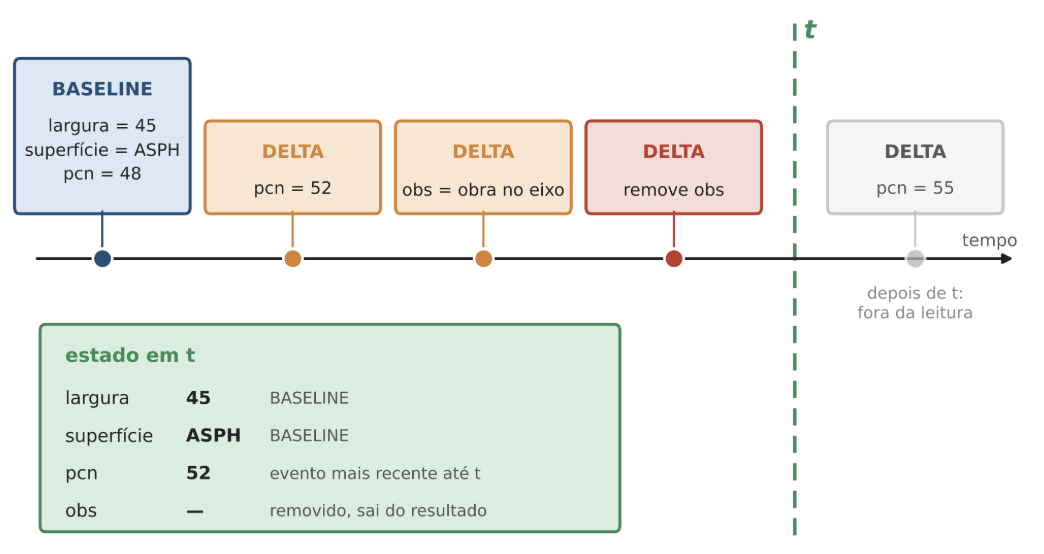
\includegraphics[width=1\linewidth]{Figures/estado-instante.png}
    \caption{Estado de uma \textit{feature} em $t$: composição do \texttt{BASELINE} com os eventos até $t$, tomando para cada caminho o valor mais recente e excluindo os campos removidos. Os valores são ilustrativos.}
    \label{fig:estado-instante}
    \par\smallskip{\small Fonte: o autor.}
\end{figure}
\subsection{Valores derivados}\label{sec:derivados}

O requisito do mínimo de informação (Seção~\ref{sec:req-minimo}) é atendido calculando na leitura tudo o que pode ser calculado. Valores como comprimento, azimute, rumo magnético e distâncias declaradas não são gravados. O comprimento e os azimutes resultam da geodésica entre os referentes, e o rumo magnético, do azimute e da variação magnética registrada no aeródromo. As distâncias declaradas resultam das definições do Anexo~14 (Seção~\ref{sec:distancias}), aplicadas ao estado no instante pedido:
\begin{equation}
    \begin{aligned}
        \mathrm{TORA} &= L, & \mathrm{TODA} &= L + \mathrm{CWY},\\
        \mathrm{ASDA} &= L + \mathrm{SWY}, & \mathrm{LDA} &= L - d,
    \end{aligned}
    \label{eq:distancias-declaradas}
\end{equation}
em que $L$ é o comprimento da pista, CWY e SWY são os comprimentos da zona livre de obstáculos e da zona de parada aplicáveis àquela direção, também calculados a partir das \textit{seeds}, e $d$ é o deslocamento da cabeceira, registrado como premissa da direção.

O cálculo é recusado, em vez de estimado, quando falta uma premissa estrutural. Sem referencial vigente, não há derivado, e uma \textit{seed} incompleta já é recusada na escrita. Pela mesma razão, um caso para o qual não há regra definida, como uma pista com barreira de contenção, leva à recusa, e não a um número possivelmente errado. Sem a norma de preenchimento proposta na Seção~\ref{sec:extensoes}, porém, o registro não distingue ``não se aplica'' de ``não informado''. A ausência de uma zona de parada, de uma zona livre de obstáculos ou de um deslocamento é lida como zero.

\subsection{Modelos de leitura e caches}

Cópias podem acelerar a leitura sem se tornar fonte de verdade. Uma delas é o estado de uma \textit{feature} ao fim de um evento, a partir do qual se aplicam apenas os eventos posteriores. Outra é o resultado de uma seleção por tipos e camadas em $t$, identificado por uma marca d'água, que é o maior \texttt{event\_id} até $t$ entre os eventos dos tipos selecionados. Um evento fora da seleção não move a marca e não invalida a cópia. Essas cópias podem ser apagadas a qualquer momento, e nenhuma escrita as lê. Um valor derivado pode, assim, ser guardado para acelerar a leitura, desde que essa cópia nunca sirva de premissa para outro cálculo.

A lente da carta de aeródromo é um exemplo de modelo de leitura. Ela monta o conteúdo de uma ADC em $t$ lendo apenas as camadas \texttt{adc} e \texttt{geometria} dos tipos que a carta mostra. Tudo o mais que o registro guarda, como os levantamentos, fica de fora sem ser lido. A tabela de distâncias da lente resulta da mesma regra da Equação~\ref{eq:distancias-declaradas}, sobre o mesmo referencial vigente. É dessa forma que se atende ao requisito de consistência entre produtos (Seção~\ref{sec:req-consistencia}). A carta e a tabela não guardam valores próprios, e duas leituras para o mesmo instante partem das mesmas afirmações.

\section{A distribuição da leitura}\label{sec:distribuicao}

Se todo produto for lido diretamente do banco, o banco passa a ser um ponto único de falha da leitura, e cada consulta concorre com a escrita. A distribuição separa as duas funções. O registro é publicado, na ordem em que foi gravado, em um único tópico, e cada consumidor monta, do seu lado, os modelos de leitura de que precisa. A Figura~\ref{fig:distribuicao} mostra o fluxo.

\begin{figure}[htbp]
    \centering
    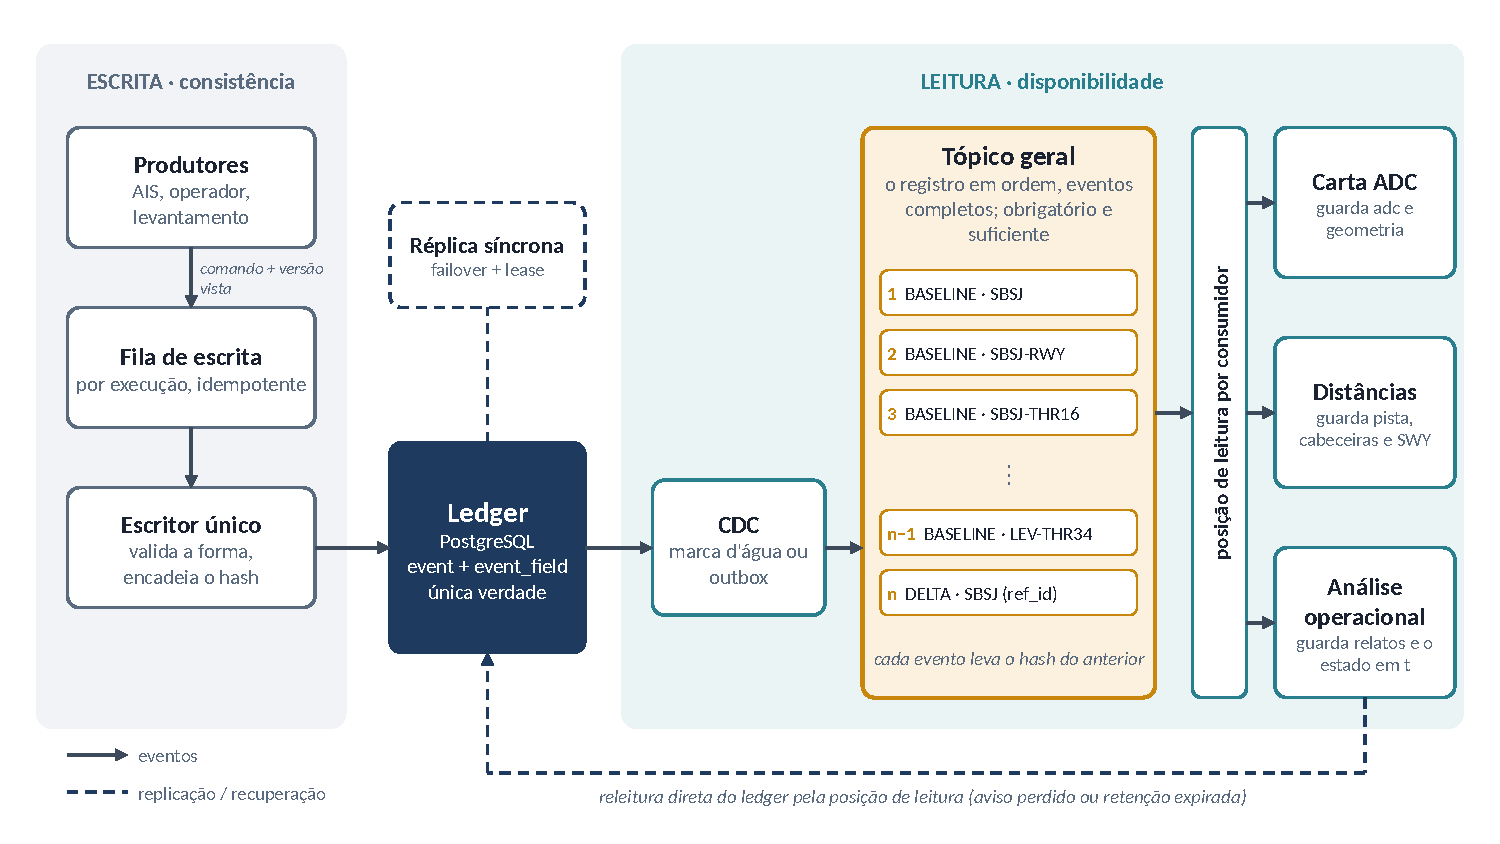
\includegraphics[width=\linewidth]{Figures/fig_arquitetura_pubsub.pdf}
    \caption{Distribuição da leitura. O registro é publicado em ordem em um tópico geral, e cada consumidor monta a sua projeção. Tudo à direita do registro é derivado e pode ser reconstruído a partir dele. A fila de escrita e a réplica síncrona, à esquerda, são extensões propostas (Seção~\ref{sec:extensoes}).}
    \label{fig:distribuicao}
    \par\smallskip{\small Fonte: o autor.}
\end{figure}

\subsection{O tópico geral}

O tópico geral é o próprio registro de um aeródromo, publicado evento a evento, com envelope e corpo, fora do banco. Ele é alimentado por um retransmissor que lê os eventos em ordem de \texttt{event\_id} e os anexa ao tópico, como em uma captura de mudanças (Seção~\ref{sec:distribuidos}). O retransmissor não guarda estado próprio, e o ponto de onde continua é o último evento já presente no tópico. Executá-lo novamente não duplica nada, e um tópico perdido é refeito do zero a partir do registro. O retransmissor também não espera nenhum consumidor. Antes do evento que adota um referencial, ele publica o corpo desse referencial, endereçado pelo conteúdo, de modo que o tópico é suficiente para quem o lê.

Há um único tópico, com todos os eventos, e todo consumidor o lê. Essa escolha mantém a camada mínima por quatro razões:
\begin{itemize}
    \item o consumidor recebe todos os eventos e, portanto, confere cada \textit{hash} e cada ligação, de ponta a ponta;
    \item os eventos de um grupo chegam juntos e em ordem, na mesma sequência, sem partes de uma mudança espalhadas por tópicos diferentes;
    \item o estado do consumidor reduz-se a uma única posição de leitura, o último evento aplicado;
    \item não há nada a rotear, e o encerramento de uma \textit{feature} é apenas mais um evento no tópico, como no registro.
\end{itemize}


\subsection{Canal não confiável}

O tópico pode estar hospedado em um intermediário que não está sob o
controle do leitor. Embora um sistema de mensageria possa tratar falhas de
entrega, como perda ou duplicação de mensagens, ele não garante que o evento
publicado esteja correto nem que seu conteúdo permaneça inalterado no
intermediário. Por isso, antes de aplicar um evento, o consumidor recalcula
seu \textit{hash}, conforme a Equação~\ref{eq:hash}, e verifica se o
\textit{hash} anterior declarado corresponde ao do último evento aplicado.
Além disso, confere se cada referencial recebido corresponde ao endereço
esperado.

Ao encontrar a primeira mensagem que falha em alguma dessas verificações,
o consumidor interrompe o processamento e não aplica nenhum evento
subsequente. Se o encadeamento de \textit{hashes} não corresponder ao
esperado, não é possível determinar, apenas com essa verificação, se o evento
recebido foi adulterado ou se a inconsistência está no último evento
aplicado. O consumidor deve, então, recuperar o último ponto de concordância
entre os eventos, caso o evento recebido permita estabelecer essa ligação,
ou descartar o último evento aplicado. Em ambos os casos, a recuperação
preserva apenas um prefixo do histórico cuja integridade não depende da
mensagem suspeita. Mensagens idênticas a eventos já aplicados são
reconhecidas como duplicatas e ignoradas.

\subsection{Consumidores}

Os consumidores são preguiçosos (\textit{lazy}) por definição. Não recebem requisições, não precisam estar sempre ativos e não precisam acompanhar o registro em tempo real. Um consumidor lê o tópico a partir da sua posição de leitura, no seu próprio ritmo, seja em laço, por agendamento ou uma única vez. Em seguida, confere e aplica o que leu e grava a nova posição. Ao ser retomado após uma queda, confere novamente o que já tinha. A Figura~\ref{fig:consumidor} mostra esse ciclo.

\begin{figure}[htbp]
    \centering
    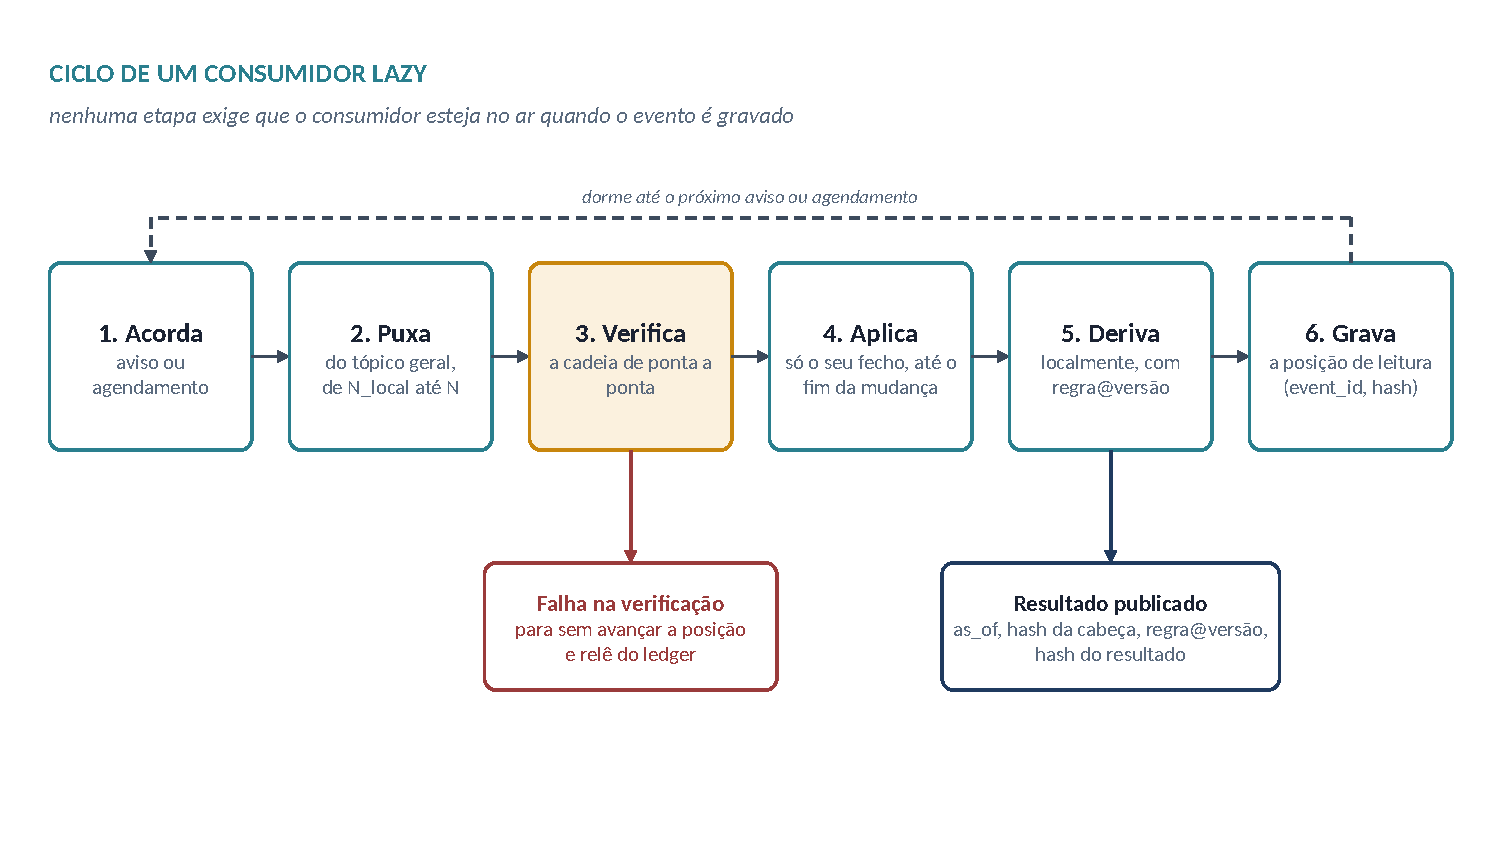
\includegraphics[width=\linewidth]{Figures/fig_ciclo_consumidor.pdf}
    \caption{Ciclo de um consumidor preguiçoso.}
    \label{fig:consumidor}
    \par\smallskip{\small Fonte: o autor.}
\end{figure}

Três regras preservam os requisitos da Seção~\ref{sec:requisitos} nesse cenário. A primeira é a do grupo inteiro, com os eventos de um grupo só são aplicados juntos, e, se o lote lido termina no meio de um grupo, o consumidor continua lendo até fechá-lo. Se o restante ainda não chegou, a posição não se move, ou seja, um corte de leitura nunca cai dentro de um grupo, e nenhuma leitura mostra uma carga pela metade.

A segunda regra é a do limite explícito. Toda leitura declara até onde vai, como \texttt{event\_id} ou como instante, e não existe leitura ``do mais recente''. Se o limite ultrapassa o que o consumidor já recebeu, ele recusa a leitura em vez de responder com um estado desatualizado.

A terceira regra é a da regra identificada. Como cada consumidor calcula os seus próprios derivados, a consistência entre produtos passa a depender de que todos apliquem a mesma regra. A regra é identificada pelo \textit{hash} do código que deriva os valores, e a resposta a declara.

\subsection{O recorte de cada consumidor}

Cada consumidor armazena todos os eventos recebidos, dado o baixo volume de
escritas, mas, ao construir uma resposta, considera apenas o fecho de
dependências das \textit{features} assinadas. Esse fecho percorre, nos dois
sentidos, as relações declaradas entre elementos, incluindo
\texttt{owner\_ref} e os campos que identificam outras \textit{features}.
Para elementos posicionados, considera também a ligação ao aeródromo, cujo
referencial determina o posicionamento. O campo \texttt{caused\_by} não
participa do fecho, pois relaciona eventos, não elementos. Relações
espaciais, como vizinhança e sobreposição, também não são armazenadas:
quando necessárias, são calculadas sobre o recorte selecionado.

Assim, a inscrição na cabeceira~16 alcança a pista, a cabeceira oposta, a
zona de parada, as restrições associadas e o aeródromo. O levantamento fica
de fora, pois sua única ligação com os demais elementos é por
\texttt{caused\_by}. Embora o aeródromo integre o fecho, suas demais relações
não são percorridas, evitando incluir todos os elementos nele posicionados.
Como todos os eventos são recebidos, novas \textit{features} que satisfaçam
essas relações, como uma barreira de contenção vinculada à pista, entram no
recorte sem exigir um mecanismo adicional de descoberta.

A resposta é um dado serializável que reúne o limite efetivo da leitura, a
cabeça da cadeia nesse limite, as \textit{features} assinadas, o fecho, os
estados, o referencial, os derivados, a regra aplicada e o \textit{hash} do
conjunto. Recusas também são representadas como respostas, na ausência de
referencial vigente, os derivados são substituídos pela indicação ``sem
referencial vigente''. Consumidores que aplicam a mesma regra ao mesmo
limite produzem o mesmo \textit{hash}; diferenças entre regras tornam as
divergências explícitas e atribuíveis, em vez de silenciosas.

\subsection{Disponibilidade e consistência}

Diante do compromisso descrito pelo teorema CAP (Seção~\ref{sec:distribuidos}), a arquitetura faz uma escolha em cada ponta. A escrita privilegia a consistência (Seção~\ref{sec:escrita}). A leitura privilegia a disponibilidade, com consumidores independentes que continuam respondendo com o banco fora do ar e que podem estar atrasados.

O atraso não leva a respostas diferentes. Como o registro só cresce, todo consumidor guarda um prefixo íntegro dele. Uma leitura com limite explícito tem, então, apenas duas respostas possíveis em qualquer consumidor. Ou seja, se ele já aplicou o registro até aquele limite, a resposta é a mesma de todos os outros; caso contrário, não há resposta. Um consumidor atrasado pode desconhecer um evento recente, mas não pode responder de forma diferente sobre um limite que já conhece.

\section{Verificação por terceiro}\label{sec:verificacao}

\subsection{Uma especificação pública}

O requisito de verificação por terceiros (Seção~\ref{sec:req-verificacao}) exige que quem recebe os dados possa conferi-los sem confiar em quem os entrega. Para isso, a especificação da cadeia (Equação~\ref{eq:hash}) é pública e curta. Qualquer pessoa pode escrever o seu próprio verificador, sem o código de quem publicou e esse verificador recalcula cada \textit{hash}, confere cada ligação e confere o identificador de cada referencial.

A mesma verificação aparece em três pontos da arquitetura. O registro verifica a si mesmo, o consumidor verifica cada mensagem do tópico, e qualquer verificador externo verifica o registro exportado e o banco extraído (Seção~\ref{sec:banco-extraido}). 

\subsection{Âncora externa}

O encadeamento denuncia qualquer alteração que deixe um sucessor. Alterar, apagar ou inserir um evento no meio do registro, ou uma mensagem no meio do tópico, quebra a cadeia a partir daquele ponto, mesmo que o atacante recalcule o \textit{hash} do evento alterado. Há, porém, alterações que não deixam sucessor para denunciá-las. No banco, é o caso de modificar apenas o último evento, truncar o final ou reescrever a cadeia inteira, recalculando todos os \textit{hashes}. No tópico, é o caso de cortar o fim, o que se confunde com atraso, ou anexar ao fim um evento falso que se liga corretamente ao último verdadeiro.

Essas alterações só são detectadas comparando a cabeça da cadeia, formada pelo último \texttt{event\_id} e pelo seu \textit{hash}, com uma âncora guardada fora do banco (Seção~\ref{sec:adulteracao}). O registro e o consumidor expõem a cabeça para esse fim, e o armazenamento e a comparação da âncora estão entre as propostas (Seção~\ref{sec:extensoes}). O encadeamento prova, portanto, que nada do que se recebeu foi alterado, mas não que se recebeu tudo.

\subsection{Cadeia linear e árvore de Merkle}

A árvore de Merkle oferece provas curtas de inclusão e de consistência (Seção~\ref{sec:adulteracao}), enquanto, na cadeia linear, o verificador refaz o percurso inteiro. Para o volume de um aeródromo, refazer o percurso tem custo baixo, e a cadeia é mais simples de especificar e de reimplementar, o que favorece justamente a verificação por terceiros. A árvore passa a valer a pena quando o registro cresce muito, ou quando é preciso provar um evento isolado a quem não deve receber o restante.

\section{O banco extraído}\label{sec:banco-extraido}

O registro é mantido em um banco servido, responsável pelas operações de
escrita e distribuição. Seu uso, entretanto, não deve depender do acesso a
esse servidor. Por isso, o produto final da arquitetura é um banco extraído:
um único arquivo SQLite~\cite{sqlite} que contém o registro completo de um
aeródromo. O banco do SBSJ é disponibilizado como conjunto de dados aberto
\cite{aeroledger_dataset}, acompanhado de cópias em CSV das principais
tabelas e visões para facilitar a inspeção.

Enquanto a AIP apresenta os valores vigentes, o banco
preserva as afirmações que lhes dão origem, incluindo autor, motivo, causa
e \textit{hash}. Dessa forma, os dados e as evidências de sua integridade
podem ser verificados por terceiros sem acesso ao banco servido, desde que
obtenham, por um canal independente, o \textit{hash} da cabeça da cadeia.

\subsection{Esquema}

O esquema espelha o do registro, com o envelope em colunas e o corpo em JSONB, o formato binário de JSON do SQLite. O arquivo contém quatro tabelas:
\begin{itemize}
    \item \texttt{exportacao}, com a procedência do arquivo e o aviso de que parte do cenário é simulada;
    \item \texttt{run}, com as cadeias contidas no arquivo;
    \item \texttt{referencial}, com o corpo de cada referencial, endereçado pelo conteúdo;
    \item \texttt{evento}, com o envelope em colunas e o corpo como a lista de linhas, cada uma com caminho, operação e valor, ordenada pelo caminho, exatamente a que entra no \textit{hash}.
\end{itemize}

Gatilhos (\textit{triggers}) do banco impedem a atualização e a exclusão de eventos, exigem o encadeamento e conferem a forma das linhas do corpo, e visões (\textit{views}) de leitura completam o arquivo. A visão \texttt{evento\_legivel} apresenta o instante extraído do próprio identificador, e a visão \texttt{campo}, o corpo achatado, com uma linha por campo. A visão \texttt{cabeca} mostra o último evento de cada cadeia, para comparação com a âncora, e a visão \texttt{estado\_atual}, as \textit{features} vivas e os seus campos. O arquivo traz ainda consultas de exemplo comentadas, que mostram o estado em um corte, o que mudou entre dois cortes, a trilha de causa de um evento e o referencial vigente. O esquema completo está no Apêndice~\ref{ape:ddl}.

Para isso, a exportação deve ser fiel, com os mesmos eventos, \textit{hashes} e cabeça do registro, e o mesmo estado em qualquer corte. Ficam fora do arquivo os derivados, que nunca são gravados, e as garantias da escrita, como a recusa de eventos malformados, que pertencem ao ponto de entrada, e não a um arquivo pronto.



\section{Implementação}\label{sec:implementacao}

A arquitetura foi implementada na biblioteca \texttt{aeroledger}, versão 0.6.0 (\textit{commit} \texttt{e93b718}) \cite{aeroledger}. A biblioteca é escrita em Python~3.12 sobre PostgreSQL~14 ou superior, com \texttt{psycopg} para o acesso ao banco, \texttt{pyproj} para a geodésia e \texttt{shapely} para a geometria. A biblioteca é o objeto avaliado. Os experimentos a utilizam como qualquer usuário a utilizaria, e cada passo corresponde a uma chamada a ela. A Tabela~\ref{tab:implementacao} relaciona as peças da arquitetura aos componentes da biblioteca.

\begin{table}[htbp]
    \centering
    \caption{Peças da arquitetura e a sua implementação no \texttt{aeroledger}.}
    \label{tab:implementacao}
    \begin{tabularx}{\linewidth}{l X}
        \toprule
        Na arquitetura & No \texttt{aeroledger} \\
        \midrule
        Escrita (Seção~\ref{sec:escrita}) & funções \texttt{escrever} e \texttt{escrever\_grupo}, que validam a forma e gravam na mesma transação \\
        Registro (Seção~\ref{sec:registro}) & tabelas \texttt{event} (envelope) e \texttt{event\_field} (uma linha por campo do corpo), apenas com inserção; tabela \texttt{referencial}, endereçada pelo conteúdo \\
        Estado em $t$ (Seção~\ref{sec:leitura}) & \texttt{DISTINCT ON} sobre o índice (\textit{feature}, caminho, evento); varredura saltada do índice para listar as \textit{features} vivas \\
        Cópias de leitura & tabelas \texttt{snapshot} e \texttt{projecao\_cache} (marca d'água) \\
        Derivados & módulo \texttt{derivacoes}; erro \texttt{RegraPendente} para a pista com barreira de contenção \\
        Lente da carta & módulo \texttt{adc} \\
        Tópico geral e consumidores (Seção~\ref{sec:distribuicao}) & módulo \texttt{topico}, com \texttt{retransmitir}, \texttt{Consumidor} e \texttt{TopicoMemoria}; erros \texttt{TopicoCorrompido} e \texttt{ConsumidorAtrasado} \\
        Verificação (Seção~\ref{sec:verificacao}) & funções \texttt{verificar\_cadeia} e \texttt{cabeca} \\
        \bottomrule
    \end{tabularx}
    \par\smallskip{\small Fonte: o autor.}
\end{table}

A implementação difere da arquitetura em quatro pontos, que limitam o alcance dos experimentos:
\begin{itemize}
    \item a escrita é serializada por um bloqueio pessimista da linha da execução (\texttt{SELECT ... FOR UPDATE}), e as formas de escrita com várias fontes da Seção~\ref{sec:extensoes} não estão implementadas;
    \item o tópico é mantido em memória (\texttt{TopicoMemoria}), com o mesmo contrato que um sistema de mensagens cumpriria, isto é, anexar e ler a partir de uma posição;
    \item a regra das distâncias declaradas com barreira de contenção não está implementada, e a biblioteca recusa o cálculo quando há uma barreira viva;
    \item o motor de geometria é uma demonstração, que desenha a carta a partir do registro, mas não foi validado contra as cartas oficiais.
\end{itemize}

A biblioteca tem 57 testes próprios, sobre um aeródromo fictício, cada um executado em um banco descartável. Eles cobrem, entre outros aspectos, as recusas de escrita, as regras do referencial, os grupos e a equivalência entre a leitura com \textit{snapshot} e a reconstrução completa. Em relação aos grupos, verificam a contiguidade, a presença no \textit{hash} e a gravação de todos ou de nenhum dos eventos. Esses testes não integram a avaliação. Eles garantem que a biblioteca faz o que declara antes de ser avaliada sobre o SBSJ.

\section{Aplicação ao SBSJ}\label{sec:aplicacao-sbsj}

\subsection{Cenário}

Os experimentos usam duas cadeias. A cadeia \texttt{aixm} guarda a pista na forma em que as publicações chegam ao usuário e serve apenas ao E1. A cadeia \texttt{sbsj} guarda a pista no modelo proposto, com os dez eventos da Tabela~\ref{tab:eventos-sbsj}, na ordem em que os experimentos os escrevem. Essa ordem compreende a carga do eAIP como um grupo de cinco eventos (E2), a remedição da cabeceira~34 trinta dias depois (E2), uma interdição de três dias (E3) e uma restrição nova escrita durante o E6. Nenhum evento contém comprimento, azimute ou distância declarada, e todos esses valores são calculados na leitura (Seção~\ref{sec:derivados}). As premissas da carga vêm da AIP. A remedição e as restrições são simuladas, para exercitar o ciclo de vida.

\begin{table}[htbp]
    \centering
    \caption{Eventos que registram a pista do SBSJ.}
    \label{tab:eventos-sbsj}
    \begin{tabularx}{\linewidth}{l l l X}
        \toprule
        \# & \textit{Feature} & Evento & Conteúdo \\
        \midrule
        1--5 & \makecell[l]{SBSJ, SBSJ-RWY,\\ SBSJ-THR16,\\ SBSJ-THR34,\\ SBSJ-SWY} & \makecell[l]{\texttt{BASELINE},\\ em grupo} & carga do eAIP: aeródromo com referencial vigente e variação magnética; pista como retângulo entre as cabeceiras, com 45~m de largura; cabeceiras sobre os seus referentes; zona de parada de 283~m além da cabeceira~34 \\
        6 & SBSJ-LEV-THR34 & \texttt{BASELINE} & levantamento que remede a cabeceira~34 (simulado) \\
        7 & SBSJ & \texttt{DELTA} & troca do referencial, com causa no evento~6 \\
        8--9 & SBSJ-RES-0001 & \makecell[l]{\texttt{BASELINE},\\ \texttt{VOID}} & interdição de 300~m a partir da cabeceira~34, com a pista como dona, e o seu encerramento (NOTAM simulado) \\
        10 & SBSJ-RES-0002 & \texttt{BASELINE} & nova restrição na pista (NOTAM simulado) \\
        \bottomrule
    \end{tabularx}
    \par\smallskip{\small Fonte: o autor, a partir de \citeonline{decea2026aip}.}
\end{table}

O referencial tem os dois referentes georreferenciados, com as coordenadas e elevações da seção AD~2.12, e o elemento linear entre eles. A pista entra como um retângulo de 45~m de largura entre as cabeceiras. A zona de parada entra como um retângulo de 283~m a partir da cabeceira~34, aplicado à direção~16. A variação magnética é de $22^\circ$W. O número 2675 não é escrito em nenhum evento.

\subsection{Procedimentos dos experimentos}\label{sec:procedimentos}

As perguntas e os critérios de aprovação de cada experimento estão na Seção~\ref{sec:experimentos}. Esta seção descreve como cada um é executado sobre o cenário.

\paragraph*{E1: causa.} A cadeia \texttt{aixm} não emula o AIXM completo, apenas as duas edições que o usuário recebe, com cada número publicado guardado como campo e sem causa. A pista é registrada com os valores da AOC de 2022 e, em seguida, alterada com os da ADC de 2026, ambos afirmados pelo DECEA. Contam-se os campos que mudam e verifica-se se algum deles traz causa.

\paragraph*{E2: derivação.} Entram no registro apenas as premissas, isto é, as coordenadas e elevações das cabeceiras, a largura da pista e as dimensões da zona de parada. O comprimento, os azimutes, os rumos magnéticos e as distâncias declaradas são calculados e comparados com os valores da AIP. Em seguida, a cabeceira~34 é remedida, deslocada em cerca de 1~m. Conferem-se então os eventos escritos e os novos valores contra o gabarito de Vincenty.

\paragraph*{E3: reconstrução no tempo.} Após a remedição, uma interdição de 300~m a partir da cabeceira~34 entra como restrição, com a pista como dona, e é encerrada três dias depois. O banco é então consultado como um auditor faria, em instantes anteriores, intermediários e posteriores a cada mudança. São consultados:
\begin{itemize}
    \item o referencial vigente e o comprimento derivado;
    \item a existência da interdição;
    \item o envelope da troca de referencial;
    \item as distâncias declaradas recalculadas para um instante passado;
    \item a diferença entre dois instantes.
\end{itemize}
O instante $t_a$, logo após a carga do eAIP, serve de referência ao longo deste e dos experimentos seguintes.

\paragraph*{E4: evidência de adulteração.} O atacante tem acesso direto ao banco. Antes dos ataques, a cabeça da cadeia é anotada fora do banco, como âncora. São executados quatro ataques:
\begin{itemize}
    \item alterar o corpo de um evento sem recalcular o \textit{hash};
    \item apagar um evento;
    \item inserir um evento com \textit{hash} próprio correto;
    \item alterar um evento e recalcular todos os \textit{hashes} até o fim.
\end{itemize}
Cada ataque é executado em uma cópia do banco e conferido de duas formas, pela verificação interna da cadeia e pela comparação com a âncora.

\paragraph*{E5: consistência e verificação.} Dois produtos são gerados do mesmo banco, antes e depois da remedição. O primeiro é a tabela da AIP, com o comprimento e as distâncias declaradas, e o segundo, o conteúdo da carta de aeródromo. Em seguida, o registro é exportado em JSON e entregue ao verificador independente, primeiro intacto e depois com a largura da pista alterada em um metro no arquivo.

\paragraph*{E6: leitura separada.} O registro é retransmitido para o tópico, e as seis propriedades do E6 são exercitadas da seguinte forma:
\begin{itemize}
    \item \textbf{equivalência}: um consumidor lê todo o tópico, e as suas respostas são comparadas com as do banco em cada fronteira de corte do histórico e em três instantes, a saber, logo após a carga, durante a interdição e um segundo antes do seu fim;
    \item \textbf{atomicidade}: o banco e o consumidor são consultados com um limite que cai dentro da carga do eAIP, logo após a pista e antes da zona de parada;
    \item \textbf{recorte}: um consumidor que assina apenas a cabeceira~16 é comparado com o que lê tudo;
    \item \textbf{limite explícito e disponibilidade}: uma restrição nova é escrita no banco, e o consumidor é consultado sobre ela antes e depois de recebê-la, e novamente com o banco fechado;
    \item \textbf{determinismo}: seis consumidores leem o tópico de formas diferentes, e comparam-se os \textit{hashes} das respostas no mesmo limite. As formas são tudo de uma vez; em laço, uma mensagem por vez; em lotes de duas mensagens, menores que a carga; por agendamento; com uma queda no meio e retomada a partir de uma posição gravada em arquivo; e a partir de um tópico refeito do zero;
    \item \textbf{canal adulterado}: o atacante está no canal, e o banco não é tocado.
\end{itemize}

No canal adulterado, o alvo é a mensagem da troca de referencial, e alterá-la equivale a fazer o tópico afirmar que o referencial antigo continua vigente. São seis ataques:
\begin{itemize}
    \item trocar o referencial sem recalcular o \textit{hash};
    \item trocar o referencial e recalcular o \textit{hash} da mensagem;
    \item remover a mensagem;
    \item inserir depois dela um evento falso com ligação e \textit{hash} corretos;
    \item remover as últimas mensagens;
    \item anexar ao fim um evento falso com ligação e \textit{hash} corretos.
\end{itemize}

\subsection{Geração do banco extraído}

O banco extraído é gerado por um programa que escreve, por meio da biblioteca, o mesmo cenário dos experimentos em um PostgreSQL vazio. Em seguida, o programa exporta o resultado para SQLite com consultas SQL diretas, sem passar pela biblioteca, e confere o arquivo com o verificador independente.

A fidelidade da exportação é verificada de três formas. A primeira é a integridade e a cabeça das duas cadeias no arquivo. A segunda é o comprimento calculado pelo verificador a partir do referencial exportado. A terceira é a consulta de estado no SQLite, feita apenas com as visões do arquivo e comparada com a da biblioteca em todos os pares de corte e \textit{feature}.

\section{Extensões propostas}\label{sec:extensoes}

A arquitetura pode ser ampliada para atender a cenários de escrita
concorrente, padronização dos dados, distribuição em maior escala, consultas
mais expressivas e verificação independente do histórico. As extensões
descritas a seguir são propostas e não foram implementadas nem avaliadas
experimentalmente. Elas preservam o registro como fonte das afirmações,
acrescentando mecanismos nas etapas de escrita, distribuição ou leitura.

\subsection{Escrita com várias fontes}

A informação aeronáutica combina dados provenientes de diferentes agentes,
como operadores de aeródromos, órgãos de informação aeronáutica e equipes
de levantamento. Para acomodar essas fontes sem comprometer a ordem do
histórico, propõe-se um escritor único por cadeia, precedido por uma fila
de comandos. Cada comando recebe uma chave de idempotência, permitindo
reconhecer reenvios e evitar gravações duplicadas. O escritor valida os
comandos, registra os eventos em sequência e confirma sua aceitação ao
remetente.

A concorrência também pode ser controlada por \textit{feature}. Para
escrever, o agente informa o último \texttt{event\_id} que observou.
Se a \textit{feature} tiver sido alterada desde então, a operação é recusada
e o agente deve consultar o estado atualizado antes de tentar novamente.
Esse controle otimista evita que uma alteração seja aceita com base em
uma versão desatualizada. Uma restrição de unicidade sobre o par formado
pela cadeia e pelo \textit{hash} anterior reforça a prevenção de bifurcações
acidentais. A versão confirmada também pode identificar o limite de leitura
e compor a chave de cache, desde que esses mecanismos utilizem a mesma
definição de versão.

\subsection{Norma de preenchimento}

A flexibilidade do registro permite acomodar diferenças entre aeródromos,
mas não determina quais informações são necessárias para validar os dados
ou calcular os derivados. Propõe-se, por isso, uma norma de preenchimento
organizada em três camadas:
\begin{itemize}
    \item uma camada obrigatória, validada na escrita, que define os tipos
    dos elementos, as unidades, a origem dos valores e os requisitos
    mínimos para o cálculo dos derivados;
    \item uma camada recomendada, baseada no catálogo de dados aeronáuticos
    do PANS-AIM~\cite{icao2018pansaim}, que padroniza nomes e unidades;
    \item uma camada de extensão, identificada pelo prefixo \texttt{x\_},
    destinada a campos específicos. Campos recorrentes podem ser
    incorporados à camada recomendada em versões posteriores da norma.
\end{itemize}

A norma distingue três estados de ausência: ``não informado'',
``não se aplica'' e ``desconhecido''. Essa distinção impede que a falta
de uma premissa seja interpretada automaticamente como zero. Por exemplo,
se o deslocamento de uma cabeceira for necessário para um cálculo, sua
ausência deve resultar na recusa desse cálculo.

A norma é versionada para que cada evento possa ser interpretado segundo
as regras aplicáveis, sem reescrever o histórico. Assim, a estrutura do
registro preserva as afirmações originais, enquanto a interpretação
padronizada pode evoluir de forma reproduzível.

\subsection{Transporte e escala}

Para o volume de dados de um único aeródromo, o próprio banco pode atender
à distribuição dos eventos. Em cenários de maior escala, um sistema de
mensageria, como o Kafka~\cite{kreps2011kafka}, pode desacoplar a escrita
do consumo e distribuir os eventos entre diferentes leitores. A adoção
desse mecanismo, entretanto, não elimina a necessidade de verificar a
integridade e a continuidade da cadeia.

Duas estratégias podem reduzir o volume transmitido. Na primeira, o tópico
transporta apenas os envelopes dos eventos, e o consumidor busca no registro
os corpos necessários ao seu recorte, conferindo cada um contra o
\textit{hash} declarado. Essa abordagem reduz o tráfego, mas mantém a
dependência de acesso ao registro.

Na segunda, tópicos derivados distribuem eventos por \textit{feature} ou
por aeródromo, permitindo segmentar o fluxo conforme as necessidades de
cada consumidor. Como esses tópicos podem omitir eventos da cadeia original,
a verificação exige informações suficientes para detectar lacunas e
confirmar a ligação dos eventos recebidos ao histórico de origem.

\subsection{Consulta}

A distribuição define como os eventos chegam ao consumidor; a consulta
define como o estado reconstruído pode ser interrogado. Uma possibilidade
é utilizar GraphQL sobre a projeção local do consumidor. Nesse modelo,
a consulta especifica o limite de leitura, seleciona o fecho de dependências
e acessa as relações declaradas e os derivados calculados segundo a regra
aplicável.

Outra possibilidade é empregar uma linguagem de consulta lógica, como
Datalog, utilizada pelo Datomic~\cite{cognitect2026}. A escolha da linguagem
determina como as perguntas são expressas, mas não altera a origem dos
dados nem as regras de reconstrução do estado. Os resultados continuam
condicionados ao histórico verificado, ao recorte selecionado, ao limite
de leitura e à regra de cálculo utilizada.

\subsection{Dois eixos de tempo}

Uma extensão bitemporal, conforme discutido na
Seção~\ref{sec:bitemporal}, permitiria distinguir o tempo de transação,
controlado pelo sistema, do tempo de validade, declarado em cada afirmação.
Com isso, seria possível consultar tanto o estado conhecido pelo sistema
em determinado instante quanto o estado correspondente a um período de
validade específico.

Essa extensão também afeta a estratégia de consulta. Enquanto o tempo de
transação permite percorrer o histórico em ordem, as consultas por intervalos
de validade podem se beneficiar de índices especializados, como um índice
GiST sobre \texttt{tstzrange} no PostgreSQL. Quando o fim de um intervalo
puder ser inferido de afirmações posteriores, ele poderá ser calculado
durante a leitura, sem alterar afirmações anteriores.

\subsection{Âncora e prova de inclusão}

Para permitir a verificação independente do histórico, propõe-se publicar
o \textit{hash} da cabeça da cadeia a cada emenda AIRAC ou depositá-lo,
junto com o banco extraído, em um repositório com histórico verificável.
A comparação com uma referência obtida por um canal independente permitiria
detectar alterações posteriores ao estado ancorado, desde que a referência
publicada não pudesse ser substituída silenciosamente.

Quando for necessário comprovar a inclusão de um evento sem compartilhar
todo o registro, uma árvore de Merkle poderá fornecer uma prova compacta
de pertencimento a um conjunto comprometido. Essa estratégia seria útil,
por exemplo, no compartilhamento seletivo de dados operacionais entre
empresas. A prova demonstraria a inclusão do evento no conjunto
correspondente, mas não garantiria a veracidade de seu conteúdo.

\section{Limites conhecidos}\label{sec:limites-arq}

As limitações a seguir dizem respeito às garantias da arquitetura
apresentada. Restrições específicas do protótipo, como funcionalidades
não implementadas e limitações de desempenho, são discutidas na
Seção~\ref{sec:implementacao}.

\begin{itemize}
    \item \textbf{Autoria:} o campo \texttt{asserted\_by} identifica o autor
    por texto, mas não comprova sua identidade, pois a arquitetura não exige
    assinatura digital.

    \item \textbf{Integridade sem âncora externa:} a cadeia de
    \textit{hashes} permite verificar a consistência interna do histórico,
    mas não impede que alguém com controle sobre todo o registro o
    reescreva. Sem uma referência independente, também não é possível
    confirmar se o histórico recebido corresponde ao anteriormente
    publicado.

    \item \textbf{Interpretação dos dados:} sem uma norma de preenchimento,
    a ausência de um campo pode ser confundida com um valor válido, como
    zero. A distinção entre ausência, inaplicabilidade e desconhecimento
    depende da adoção de convenções explícitas.

    \item \textbf{Confidencialidade:} o tópico geral expõe os eventos nele
    publicados aos seus consumidores. O isolamento de dados restritos exige
    mecanismos adicionais, como fluxos separados e controles de acesso.
    A publicação de \textit{hashes}, isoladamente, não garante
    confidencialidade.

    \item \textbf{Escopo temporal e espacial:} cada cadeia representa um
    único aeródromo, e a ordenação de eventos entre aeródromos distintos
    não é definida. Além disso, o modelo atual utiliza apenas o tempo de
    transação; consultas pelo tempo de validade exigem uma extensão
    bitemporal.

    \item \textbf{Banco extraído:} o arquivo preserva o histórico registrado,
    mas não inclui necessariamente os derivados nem impede modificações
    diretas. Sua integridade depende de verificações realizadas sobre o
    conteúdo e de uma referência confiável para comparação.

    \item \textbf{Veracidade:} a integridade do histórico não garante que
    as medições estejam corretas. A arquitetura permite rastrear quem
    afirmou um valor, quando a afirmação foi registrada e de quais dados
    ela depende, mas a validação factual exige fontes e procedimentos
    externos.
\end{itemize}